\chapter{RDF Schema}
\label{ch8}

Just as Semantic Web modeling in RDF is about graphs, Semantic Web
modeling in the RDF Schema Language (RDFS) is about sets. Some aspects
of set membership can be modeled in RDF alone, as we have seen with the
\texttt{rdf:type} built-in property. But RDF itself simply creates a graph
structure to represent data. RDFS provides some guidelines about how to
use this graph structure in a disciplined and standardized way. It
provides a way to talk about the vocabulary that will be used in an RDF
graph. Which individuals are related to one another, and how? How are
the properties we use to define our individuals related to other sets of
individuals and, indeed, to one another? RDFS provides a way for an
information modeler to express the answers to these sorts of questions
as they pertain to particular data modeling and integration needs.

As such, RDFS is like other schema languages: It provides information
about the ways in which we describe our data. But RDFS differs from
other schema languages in important ways.

\section{Schema Languages and their Functions}

RDFS is the schema language for RDF. But what is a schema language in
the first place? There are a number of successful schema languages for
familiar technologies, but the role that each of these languages play in
the management of information is closely tied to the particular language
or system.

Let's consider document modeling systems as an example. For such a
system, a schema language allows one to express the set of allowed
formats for a document. For a given schema, it is possible to determine
(often automatically) whether a particular document conforms to that
schema. This is the major capability provided by XML Schema definitions.
XML parsers can automatically determine whether a particular XML
document conforms to a given schema.

Other schema languages help us to interpret particular data. For
example, a database schema
provides header and key information for tables in a relational database.
There is neither anything in the table itself to indicate the meaning of
the information in a particular column nor anything to indicate which
column is to be used as an index for the table. This information is
appropriately included in the database schema, since it does not change
from one data record to the next.

For Object-Oriented Programming systems, the class structure plays an
organizing role for information as well. But in object-oriented
programming, the class diagram does more than describe data. It
determines, according to the inheritance policy of the particular
language, what methods are available for a particular instance and how
they are implemented. This stands in stark contrast to relational
databases and XML, in that it does not interpret information but instead
provides a systematic way for someone to describe information and
available transformations for that information.

Given this variety of understandings of how schema information can be
used in different modeling paradigms, one might wonder whether calling
something a schema language actually tells us anything at all! But there
is something in common among all these notions of a schema. In all
cases, the schema tells us something about the information that is
expressed in the system. The schema is information about the data.

How then can we understand the notion of schema in RDF? What might we
want to say about RDF data? And how might we want to say it? The key
idea of the schema in RDF is that it should help provide some sense of
meaning to the data. It accomplishes this by specifying semantics using
inference patterns.

\subsection{Relationship between schema and data}

In most modeling systems, there is a clear division between the data and
its schema. The schema for a relational database is not typically
expressed in a table in the database; the object model of an
object-oriented system is not expressed as objects, and an XML DTD \footnote{DTD was the original document type definition format for XML} is
not a valid XML document.

But in many cases, modern versions of such systems do model the schema
in the same form as the data; the meta-object protocol of Common Lisp
and the introspection API of Java represent the object models as objects
themselves. The XML Stylesheet Definition (XSD) \footnote {XSD is the modern way to define XML schemas} defines XML Styles in an XML
language.

In the case of RDF, the schema language was defined in RDF from the very
beginning. That is, all schema information in RDFS is defined with RDF
triples. The relationship between ``plain'' resources in RDF and schema
resources is made with triples, just like relationships between any
other resources. This elegance of design makes it particularly easy to
provide a formal description of the semantics of RDFS, simply by
providing inference rules that work over patterns of triples. While this
is good engineering practice (in some sense, the RDF standards committee
learned a lesson from the issues that the XML standards had with DTDs),
its significance goes well beyond its value as good engineering. In RDF,
everything is expressed as triples. The meaning of asserted triples is
expressed in new (inferred) triples. The structures that drive these
inferences, that describe the meaning of our data, are also in triples.
This means that this process can continue as far as it needs to; the
schema information that provides context for information on the Semantic
Web can itself be distributed on the Semantic Web. This also means that
every tool and technique available for RDF data is available for RDFS
schemata: you can query a schema in SPARQL, validate it in SHACL, edit
it in an RDF editor, publish it with Linked Data practices and tools,
visualize it with an RDF visualizer, etc.

We can see this in action by showing how a set is defined in RDFS. The
basic construct for specifying a set in RDFS is called an \texttt{rdfs:Class}.
Since RDFS is expressed in RDF, the way we express that something is a
class is with a triple---in particular, a triple in which the predicate
is \texttt{rdf:type}, and the object is \texttt{rdfs:Class}. Here are some examples that
we will use in the following discussion:

\begin{lstlisting}
:AllStarPlayer rdf:type rdfs:Class .
:MajorLeaguePlayer rdf:type rdfs:Class .
:Surgeon rdf:type rdfs:Class .
:Staff rdf:type rdfs:Class .
:Physician rdf:type rdfs:Class .
\end{lstlisting}

These are triples in RDF just like any other; the only way we know that
they refer to the schema rather than the data is because of the use of
the term in the \texttt{rdfs:} namespace, \texttt{rdfs:Class}. But what is new here? In
Chapter~\ref{ch3}, we already discussed the notion of \texttt{rdf:type}, which we used to
specify that something was a member of a set. What do we gain by
specifying explicitly that something is a set? We gain a description of
the meaning of membership in a set. In RDF, the only ``meaning'' we had
for set membership was given by the results of some query; \texttt{rdf:type}
actually didn't behave any differently from any other (even
user-defined) property. How can we specify what we mean by set
membership? In RDFS, we express meaning through the mechanism of
inference.

\section{The RDF Schema Language}

RDFS ``extends'' RDF by introducing a set of distinguished resources
into the language. This is similar to the way in which a traditional
programming language can be extended by defining new language- defined
keywords. But there is an important difference: In RDF, we already had
the capability to use

any resource in any triple (Anyone can say Anything about Any topic). So
by identifying certain specific resources as ``new keywords,'' we
haven't actually extended the language at all! We have simply identified
certain triples as having a special meaning, as defined by a standard.

How can we define the ``meaning'' of a distinguished resource? As we saw
in Chapter~\ref{ch7}, in RDFS, meaning is expressed by specifying inferences
that can be drawn when the resource is used in a certain way. Throughout
the rest of this section, whenever we introduce a new RDFS resource, we
will answer the question ``What does it mean?'' with an answer of the
form ``In these circumstances (defined by some pattern of triples), you
can add (infer) the following new triples.'' We already saw how to do
this with the type propagation rule for \texttt{rdfs:subClassOf}; now we will
demonstrate this principle using another of the most fundamental terms
in RDFS: \texttt{rdfs:subPropertyOf}.

\subsection{Relationship propagation through rdfs:subPropertyOf}

The basic intuition behind the use of \texttt{rdfs:subPropertyOf} is that
terminology includes verbs as well as nouns, and many of the same
requirements for mapping nouns from one source to another will apply to
relationships. Simple examples abound in ordinary parlance. The
relationship brother is more specific than the relationship sibling; if
someone is my brother, then he is also my sibling. This is formalized in
RDFS for \texttt{rdfs:subPropertyOf} using an inference rule that is almost as
simple as the one for \texttt{rdfs:subClassOf}.

\begin{lstlisting}
CONSTRUCT {?x ?r ?y .}
WHERE {?x ?q ?y .
       ?q rdfs:subPropertyOf ?r }
\end{lstlisting}

That is, in any triple, we can replace the predicate with any property
it is a \texttt{subPropertyOf}.

\begin{example}{Employment}

A large firm engages a number of people in various capacities and has a
variety of ways to administer these relationships. Some people are
directly employed by the firm, whereas others are contractors. Among
these contractors, some of them are directly contracted to the company
on a freelance basis, others on a long-term retainer, and still others
contract through an intermediate firm. All of these people could be said
to work for the firm.

How can we model this situation in RDFS? First, we need to consider the
inferences we wish to be able to
draw and under what circumstances. There are a number of relationships
that can hold between a person and the firm; we can call them
\texttt{contractsTo}, \texttt{freeLancesTo}, \texttt{indirectlyContractsTo}, \texttt{isEmployedBy}, and
\texttt{worksFor}.

If we assert any of these statements about some person, then we would
like to infer that that person
\texttt{worksFor} the firm. Furthermore, there are intermediate conclusions we
can draw---for instance, both a freelancer and an indirect contractor
contract to the firm and indeed work for the firm.

All these relationships can be expressed in RDFS using the
\texttt{rdfs:subPropertyOf} relation:

\begin{lstlisting}
:freeLancesTo rdfs:subPropertyOf contractsTo .
:indirectlyContractsTo rdfs:subPropertyOf contractsTo .
:isEmployedBy rdfs:subPropertyOf worksFor .
:contractsTo rdfs:subPropertyOf worksFor .
\end{lstlisting}

\begin{figure}
\centering
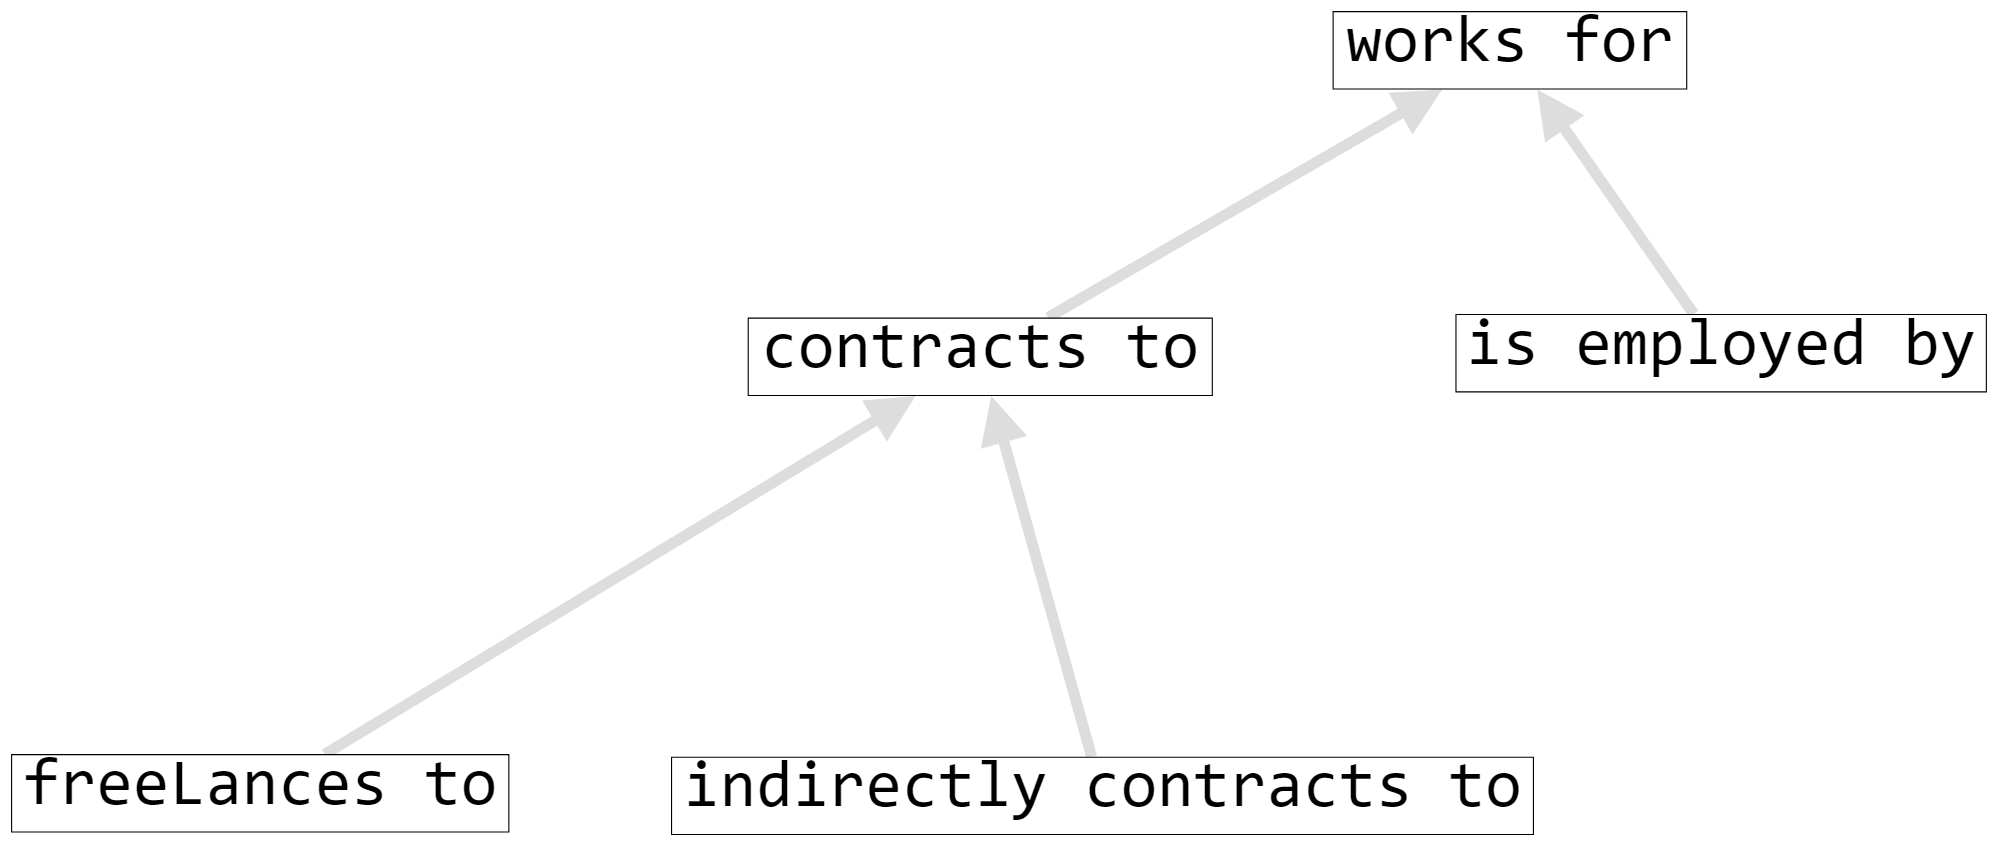
\includegraphics[width=5in]{SWWOv3/media/ch8/figure8-1.png}
\caption{rdfs:subPropertyOf relations for workers in the firm.}
\label{fig:ch8.1}
\end{figure}


The discussion will be easier to follow if we represent this as a
diagram, where the arrows denote
\texttt{rdfs:subPropertyOf} (see Figure~\ref{fig:ch8.1}).

To see what inferences can be drawn, we will need some instance data:

\begin{lstlisting}
:Goldman :isEmployedBy :TheFirm .
:Spence :freeLancesTo :TheFirm .
:Long :indirectlyContractsTo :TheFirm .
\end{lstlisting}

The rule that defines the meaning of \texttt{rdfs:subPropertyOf} implies a new
triple, replacing any sub- property with its superproperty. So, since

\begin{lstlisting}
:isEmployedBy :rdfs:subPropertyOf :worksFor.
\end{lstlisting}

we can infer that

\begin{lstlisting}
* :Goldman :worksFor :TheFirm.
\end{lstlisting}

And because of the assertions about freelancing and indirect contracts,
we can infer that

\begin{lstlisting}
* :Spence :contractsTo :TheFirm .
* :Long contractsTo :TheFirm .
\end{lstlisting}

And finally, since, like asserted triples, inferred triples can be used
to make further inferences, we can further infer that

\begin{lstlisting}
* :Spence :worksFor :TheFirm .
* :Long :worksFor :TheFirm .
\end{lstlisting}

In general, \texttt{rdfs:subPropertyOf} allows a modeler to describe a hierarchy
of related properties. Just as in class hierarchies, specific properties
are at the bottom of the tree, and more general properties are higher up
in the tree. Whenever any property in the tree holds between two
entities, so does every property above it.
\end{example}

\begin{sidebar}{OO Comparison}
The construct \texttt{rdfs:subPropertyOf} has no direct analog in object-oriented
programming, where properties are not first-class entities (i.e., they
cannot be related to one another, independent of the class in which they
are defined). For this reason, unlike the case of \texttt{rdfs:subClassOf},
object-oriented programmers have no conflict with a similar known
concept. The only source of confusion is that subproperty diagrams like
the preceding one are sometimes mistaken for class diagrams.
\end{sidebar}

\subsection{Typing data by usage---rdfs:domain and rdfs:range}
\label{section:domainrange}

We have seen how inferences around \texttt{rdfs:subPropertyOf} can be used to
describe how two properties relate to each other. But when we describe
the usage of terms in our data, we would also like to represent how a
property is used relative to the defined classes. In particular, we
might want to say that when a property is used, the triple subject comes
from (i.e., has \texttt{rdf:type}) a certain class and that the object comes from
some other type. These two stipulations are expressed in RDFS with the
resources (keywords) \texttt{rdfs:domain} and \texttt{rdfs:range}, respectively.

In mathematics, the words \emph{domain} and \emph{range} (or \emph{co-domain}) are used to
refer to how a function (or more generally, a relation) can be used. The
domain of a function is the set of values for which it is defined, and
the range is the set of values it can take. In Real Analysis, for
instance, the relation \emph{squareroot} has the positive numbers as the domain
(since negative numbers don't have square roots in the reals), and all
reals as the range (since there are both positive and negative square
roots).

In RDFS, the properties \texttt{rdfs:domain} and \texttt{rdfs:range} have meanings
inspired by the mathematical uses of these words. A property p can have
an \texttt{rdfs:domain} and/or an \texttt{rdfs:range}. These are specified, as is
everything in RDF, via triples:

\begin{lstlisting}
:p rdfs:domain :D.
:p rdfs:range :R.
\end{lstlisting}

The informal interpretation of this is that the relation \texttt{p} relates
values from the class \texttt{D} to values from the class \texttt{R}. \texttt{D} and \texttt{R} need not be
disjoint, or even distinct.

The meaning of these terms is defined by the inferences that can be
drawn from them. RDFS
inferencing interprets domain with the inference rule:

\begin{lstlisting}
CONSTRUCT {?x rdf:type ?D .}
WHERE {?P rdfs:domain ?D .
       ?x ?P ?y .}
\end{lstlisting}

Similarly, range is defined with the rule

\begin{lstlisting}
CONSTRUCT {?y rdf:type ?D .}
WHERE {?P rdfs:range ?D .
       ?x ?P ?y .}
\end{lstlisting}

In RDFS, domain and range give some information about how the property P
is to be used; domain refers to the subject of any triple that uses P as
its predicate, and range refers to the object of any such triple. When
we assert that property P has domain D (respectively, range R), we are
saying that whenever we use the property P, we can infer that the
subject (respectively object) of that triple is
a member of the class D (respectively R). In short, domain and range
tell us how P is to be used. Rather than signaling an error if P is used
in a way that is apparently inconsistent with this declaration, RDFS
will infer the necessary type information to bring P into compliance
with its domain and range declarations.

In RDFS, there is no way to assert that a particular individual is not a
member of a particular class (contrast with OWL, Chapter~\ref{ch13}). In fact,
in RDFS, there is no notion of an incorrect or inconsistent inference.
This means that, unlike the case of XML Schema or SHACL shape, an RDF
Schema will never proclaim an input as invalid; it will simply infer
appropriate type information. In this way, RDFS behaves much more like a
database schema, which declares what joins are possible but makes no
statement about the validity of the joined data.

\subsection{Combination of domain and range with rdfs:subClassOf}

So far, we have seen inference patterns for some resources in the rdfs
namespace: \texttt{rdfs:domain}, \texttt{rdfs:range}, \texttt{rdfs:subPropertyOf}, and
\texttt{rdfs:subClassOf}. We have seen how the inference patterns work on sample
triples. But the inference patterns can also interact with one another
in interesting ways. We can already see this happening with the three
patterns we have seen so far. We will show the interaction between
\texttt{rdfs:subClassOf} and \texttt{rdfs:domain} by starting with an example.

Suppose we have a very simple class tree that includes just two classes,
\texttt{Woman} and \texttt{MarriedWoman}, in the usual subclass relation:

\begin{lstlisting}
:MarriedWoman rdfs:subClassOf :Woman.
\end{lstlisting}

Suppose we have a property called \texttt{hasMaidenName}, whose domain is
\texttt{MarriedWoman}:

\begin{lstlisting}
:hasMaidenName rdfs:domain :MarriedWoman.
\end{lstlisting}

Figure\ref{fig:ch8.2} shows how this looks in diagram form.

\begin{figure}
\centering
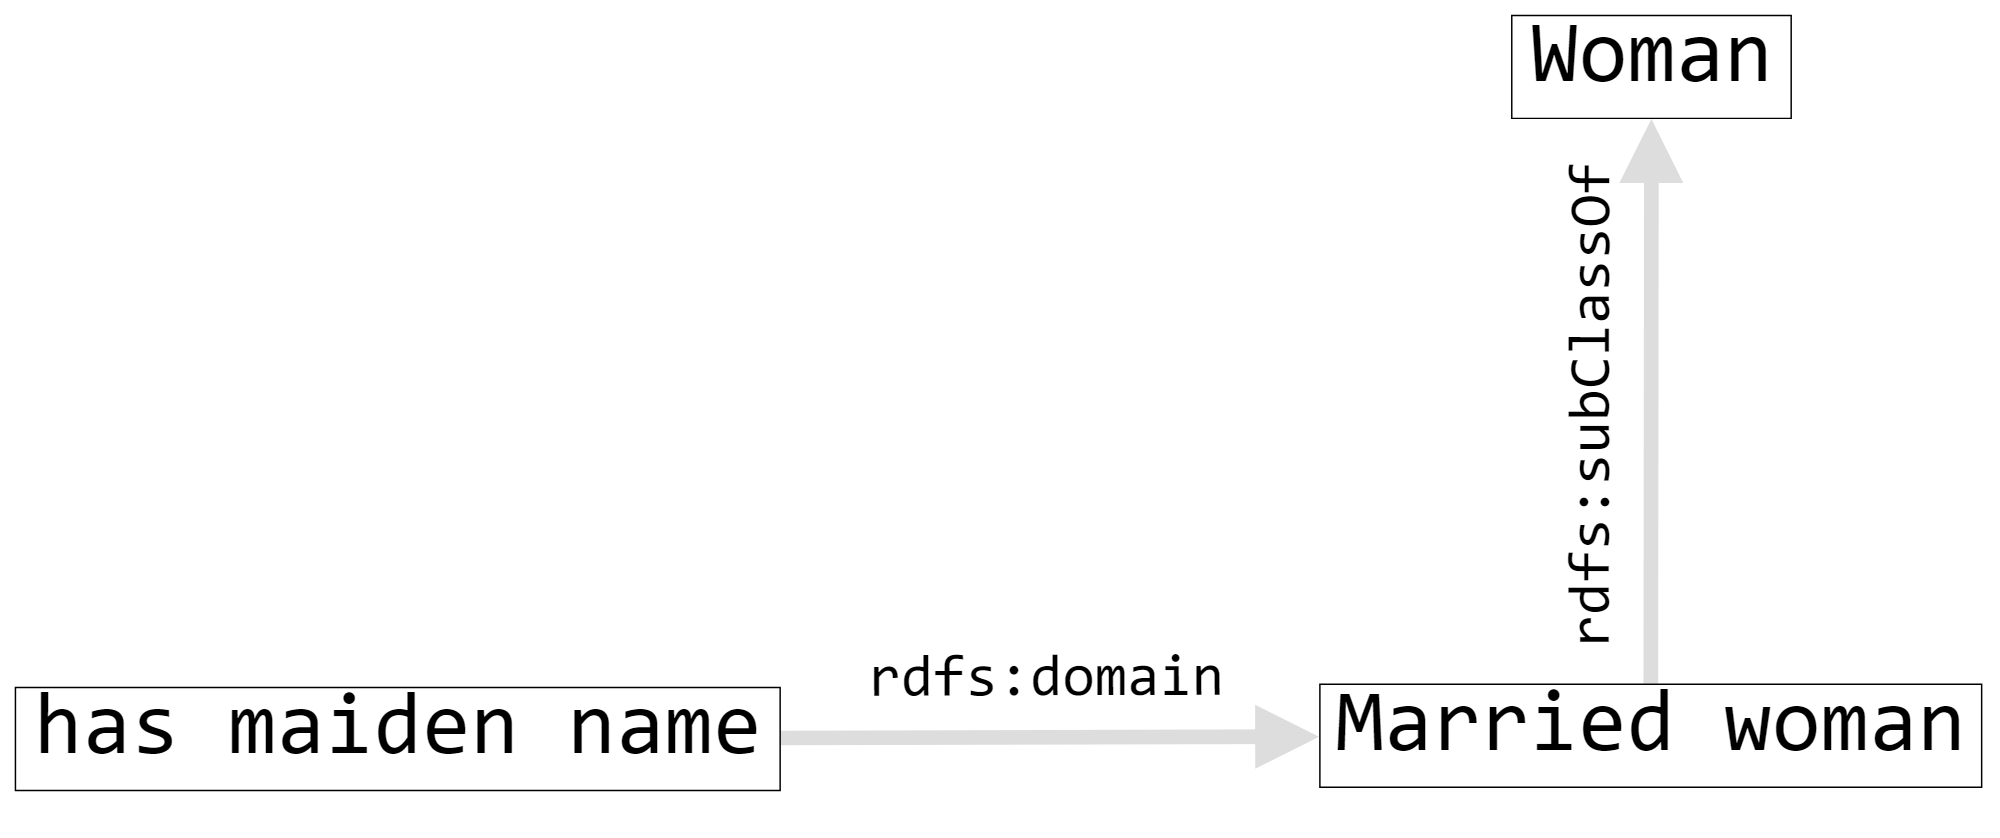
\includegraphics[width=5in]{SWWOv3/media/ch8/figure8-2.png}
\caption{Domain and subClassOf triples for hasMaidenName.}
\label{fig:ch8.2}
\end{figure}


This unsurprising model holds some subtlety; let's examine closely what
it says. If we assert the \texttt{hasMaidenName} of anything (even if we don't
know that it is a \texttt{Woman}!), the rule for \texttt{rdfs:domain} allows us to infer
that it is a \texttt{MarriedWoman}. So, for instance, if someone asserts

\begin{lstlisting}
:Karen :hasMaidenName :MarriedWoman.
\end{lstlisting}

We can infer

\begin{lstlisting}
* :Karen rdf:type :MarriedWoman.
\end{lstlisting}

But we can make further inferences based on the \texttt{rdfs:subClassOf}
relationship between the classes---namely, that

\begin{lstlisting}
* :Karen rdf:type :Woman.
\end{lstlisting}

There was nothing in this example that was particular to Karen; in fact,
if we learn of any resource at all that it has a \texttt{hasMaidenName}, then we
will infer that it is a \texttt{Woman}. That is, we know that for any resource X,
if we have a triple of the form

\begin{lstlisting}
?X :hasMaidenName ?Y .
\end{lstlisting}

we can infer

\begin{lstlisting}
* ?X rdf:type :Woman.
\end{lstlisting}

But this is exactly the definition of \texttt{rdfs:domain}; that is, we have just
seen that

\begin{lstlisting}
:hasMaidenName rdfs:domain :Woman.
\end{lstlisting}

This is a different way to use the definition of \texttt{rdfs:domain} from what
we have encountered so far. Until now, we applied the inference pattern
whenever a triple using \texttt{rdfs:domain} was asserted or inferred. Now we are
inferring an \texttt{rdfs:domain} triple whenever we can prove that the inference
pattern holds. That is, we view the inference pattern as the definition
of what it means for \texttt{rdfs:domain} to hold.

We can generalize this result to form a new inference pattern as
follows:

\begin{lstlisting}
CONSTRUCT {?P rdfs:domain ?C .}
WHERE {?P rdfs:domain ?D .
       ?D rdfs:subClassof ?C .}
\end{lstlisting}

That is, whenever we specify the \texttt{rdfs:domain} of a property to be some
class, we can also infer that the property also has any superclass as
\texttt{rdfs:domain}. The same conclusion holds for \texttt{rdfs:range}, using the same
argument.

These simple definitions of domain and range are actually quite
aggressive; we can draw conclusions about the type of any element based
simply on its use in a single triple whenever we have domain or range
information about the predicate. As we shall see in later examples, this
can result in some surprising inferences. The definitions of domain and
range in RDFS are the most common problem areas for modelers with
experience in another data modeling paradigm. It is unusual to have such
a strong interpretation for very common concepts.

\begin{sidebar}{}
The interaction between \texttt{rdfs:domain} and \texttt{rdfs:subClassOf} can seem
particularly counterintuitive when viewed in comparison to
Object-Oriented Programming (OOP). One of the basic mechanisms for
organizing code in OOP is called inheritance. There are a number of
different schemes for defining inheritance, but they typically work by
propagating information down the class tree; that is, something (e.g., a
method or a variable) that is defined at one class is also available at
its subclasses.

When they first begin working with RDFS, there is a tendency for OO
programmers to expect inheritance to work the same way. This tendency
results from an ``obvious'' mapping from RDFS to OOP in which an
\texttt{rdfs:Class} corresponds to a Class in OOP, a property in RDFS corresponds
to a variable in OOP, and in which the assertion

\begin{lstlisting}
P rdfs:domain C.
\end{lstlisting}

corresponds to the definition of the variable corresponding to P being
defined at class C. From this ``obvious'' mapping comes an expectation
that these definitions should inherit in the same way that variable
definitions inherit in OOP.

But in RDFS, there is no notion of inheritance per se; the only
mechanism at work in RDFS is inference. The inference rule in RDFS that
most closely corresponds to the OO notion of inheritance is the subclass
propagation rule: that the members of a subclass are also members of a
class. The ramifications of this rule for instance correspond to what
one would expect from inheritance. Since an instance of a subclass is
also an instance of the parent class, then anything we say about members
of the parent class will necessarily hold for all instances of the
subclass; this is consistent with usual notions of inheritance.

The interaction between \texttt{rdfs:domain} and \texttt{rdfs:subClassOf}, on the other
hand, is more problematic. Using the ``obvious'' interpretation, we
asserted that the variable \texttt{hasMaidenName} was defined at \texttt{MarriedWoman} and
then inferred that it was defined at a class higher in the
tree---namely, \texttt{Woman}. Seen from an OO point of view, this interaction
seems like inheritance up the tree---in other words, just the opposite
of what is normally expected of inheritance in OOP.

The fallacy in this conclusion comes from the ``obvious'' mapping of
\texttt{rdfs:domain} as defining a variable relative to a class. In the Semantic
Web, because of the AAA slogan, a property can be used anywhere, and it
must be independent of any class. The property \texttt{hasMaidenName} was, by
design, always available for any resource in the universe (including
members of the class \texttt{Woman}); the assertion or inference of \texttt{rdfs:domain}
made no change in that respect. That is, it is never accurate in the
Semantic Web to say that a property is ``defined for a class.'' A
property is defined independently of any class, and the RDFS relations
specify which inferences can be correctly made about it in particular
contexts.

\end{sidebar}

\section{RDFS Modeling Combinations and Patterns}

The inference rules for RDFS are few in number and quite simple.
Nevertheless, their effect can be quite subtle in the context of shared
information in the Semantic Web. In this section, we outline a number of
patterns of use of the basic RDFS features, illustrating each one with a
simple example.

\subsection{Set intersection}
\label{sintersection}

It is not uncommon for someone modeling in RDFS to ask whether some
familiar notions from logic are available. ``Can I model set
intersection in RDFS?'' is a common question. The technically correct
answer to this question is simply ``no.'' There is no explicit modeling
construct in RDFS for set intersection (or for set union). However, when
someone wants to model intersections (or unions), they don't always need
to model them explicitly. They often only need certain particular
inferences that are
supported by these logical relations. Sometimes these inferences are
indeed available in RDFS through particular design patterns that combine
the familiar RDFS primitives in specific ways.

In the case of intersection in particular, one of the inferences someone
might like to draw is that if a resource x is in C, then it is also in
both A and B. Expressed formally, the relationship they are expressing
is that $C \subseteq A \cap B$. This inference can be supported by making C a common
subclass of both A and B, as follows:

\begin{lstlisting}
:C rdfs:subClassOf :A.
:C rdfs:subClassOf :B.
\end{lstlisting}

How does this support an intersection-like conclusion? From the
inference rule governing
\texttt{rdfs:subClassOf}, it is evident that from the triple

\begin{lstlisting}
?x rdf:type :C.
\end{lstlisting}


We can infer

\begin{lstlisting}
?x rdf:type :B .
?x rdf:type :A .
\end{lstlisting}

as desired. Notice that we can only draw the inferences in one
direction; from membership in C, we can infer membership in A and B. But
from membership in A and B, we cannot infer membership in C. That is, we
cannot express $A \cap B \subseteq C$. This is the sense in which RDFS cannot
actually express set intersection; it can only approximate it by
supporting the inferencing in one direction.

\begin{example}{Hospital Skills}

Suppose we are describing the staff at a hospital. There are a number of
different jobs and people who fill them, including nurses, doctors,
surgeons, administrators, orderlies, volunteers, and so on. A very
specialized role in the hospital is the surgeon. Among the things we
know about surgeons is that they are members of the hospital staff. They
are also qualified physicians. Logically, we would say that $ \texttt{Surgeon}  \subseteq
\texttt{Staff} \cap \texttt{Physician}$ --- that is, Surgeon is a subset of those people who are
both staff members and physicians.

Notice that we don't want to say that every staff physician is a
surgeon, so the set inclusion goes only one
way. From this statement, we want to be able to infer that if Kildare is
a Surgeon, then he is also a member of the staff, and he is a physician.
If we say

\begin{lstlisting}
:Surgeon rdfs:subClassOf :Staff .
:Surgeon rdfs:subClassOf :Physician .
:Kildare rdf:type :Surgeon .
\end{lstlisting}

then we can infer that

\begin{lstlisting}
* :Kildare rdf:type :Staff .
* :Kildare rdf:type :Physician .
\end{lstlisting}

We cannot make the inference the other way; that is, if we were to
assert that Kildare is a Physician and
member of the Staff, no RDFS rules are applicable, and no inferences are
drawn. This is appropriate; consider the case in which Kildare is a
psychiatrist. As such, he is both a member of the Staff and a Physician,
but it is inappropriate to conclude that he must be a Surgeon. (OWL,
Chapter~\ref{ch13}, provides a way to state axioms so that this  conclusion could
hold, but RDFS does not.)
\end{example}

\subsection{Property intersection}
\label{pintersection}
In RDFS, properties are treated in a way analogous to the treatment of
classes, and all the same operations and limitations apply. Even though
it might seem unfamiliar to think of a property as a set, we can still
use the set combination terms (intersection, union) to describe the
functionality supported for properties. As was the case for Class
intersections and unions, RDFS cannot express these things exactly, but
it is possible to approximate these notions with judicious use of
\texttt{subPropertyOf}.

One of the inferences we can express using \texttt{subPropertyOf} is that one
property is an intersection
of two others, $P \subseteq R \cap S$. That is, if we know that two resources x and y
are related by property P,

\begin{lstlisting}
?x :P ?y .
\end{lstlisting}

we want to be able to infer both

\begin{lstlisting}
?x :R ?y .
?x :S ?y.
\end{lstlisting}

\begin{example}{Patients in Hospital Rooms}

Suppose we are describing patients in a hospital. When a patient is
assigned to a particular room, we can infer a number of things about the
patient: We know that they are on the duty roster for that room and that
their insurance will be billed for that room. How do we express that
both of these inferences come from the single assignment of a patient to
a room?

\begin{lstlisting}
:lodgedIn rdfs:subPropertyOf :billedFor.
:logdedIn rdfs:subPropertyOf :assignedTo.
\end{lstlisting}

Now if patient Marcus is lodged in Room 101,

\begin{lstlisting}
:Marcus :lodgedIn :Room101 .
\end{lstlisting}

we can infer the billing and duty roster properties as well:

\begin{lstlisting}
* :Marcus :billedFor :Room101 .
* :Marcus :assignedTo :Room101 .
\end{lstlisting}

Notice that we cannot make the inference in the other direction; that
is, if we were to assert that Marcus is billedFor Room101 and assignedTo
Room101, no RDFS rules are applicable, and no inferences can be drawn.
\end{example}


\subsection{Set Union}
\label{sunion}
Using a pattern similar to the one we used for set intersection, we can
also express certain things about set unions in RDFS. In particular, we
can express that $A \cup B \subseteq C$. We do this by making C a common superclass
of A and B, thus:

\begin{lstlisting}
:A rdfs:subClassOf :C.
:B rdfs:subClassOf :C.
\end{lstlisting}

Any instance ?x that is a member of either A or B is inferred to be also
a member of C; that is,

\begin{lstlisting}
?x rdf:type :A.
\end{lstlisting}

or

\begin{lstlisting}
?x rdf:type :B.
\end{lstlisting}

implies

\begin{lstlisting}
* ?x rdf:type :C.
\end{lstlisting}

\begin{example}{All Stars}

In determining the candidates for a season's All Stars, a league's rules
could state that they will select among all the players who have been
named Most Valuable Player (\texttt{MVP}), as well as among those who have been
top scorers (\texttt{TopScorer}) in their league. We can model this in RDFS by
making \texttt{AllStarCandidate} a common superclass of \texttt{MVP} and \texttt{TopScorer} as
follows:

\begin{lstlisting}
:MVP rdfs:subClassOf :AllStarCandidate.
:TopScorer rdfs:subClassOf :AllStarCandidate.
\end{lstlisting}

Now, if we know that Reilly was named MVP and Kaneda was a TopScorer:

\begin{lstlisting}
:Reilly rdf:type :MVP .
:Kaneda rdf:type :TopScorer .
\end{lstlisting}

then we can infer that both of them are AllStarCandidates

\begin{lstlisting}
* :Reilly rdf:type :AllStarCandidate .
* :Kaneda rdf:type :AllStarCandidate .
\end{lstlisting}

as desired. Notice that as in the case of intersection, we can only draw
the inference in one direction---that is, we can infer that
$\texttt{AllStarCandidate} \supseteq \texttt{MVP} \cup \texttt{TopScorer}$, but not the other way around.

In summary, we can use \texttt{rdfs:subClassOf} to represent statements about
intersection and union as
follows:

\begin{itemize}
\item $C \subseteq A \cap B$ (by making C rdfs:subClassOf both A and B)

\item $C \supseteq  A \cup B$ (by making both A and B rdfs:subClassOf C).
\end{itemize}
\end{example}

\subsection{Property union}
\label{punion}
One can use \texttt{rdfs:subPropertyOf} to combine properties from different
sources in a way that is analogous to the way in which \texttt{rdfs:subClassOf}
can be used to combine classes as a (pseudo-)union. If two different sources use
properties P and Q in similar ways, then a single amalgamated property R
can be defined with \texttt{rdfs:subPropertyOf} as follows:

\begin{lstlisting}
:P rdfs:subPropertyOf :R .
:Q rdfs:subPropertyOf :R .
\end{lstlisting}

For any pair of resources x and y related by P or by Q

\begin{lstlisting}
?x :P ?y .
\end{lstlisting}

or

\begin{lstlisting}
?x :Q ?y .
\end{lstlisting}

we can infer that

\begin{lstlisting}
* ?x :R ?y .
\end{lstlisting}

\begin{example}{Merging Library Records}

Suppose one library has a table in which it keeps lists of patrons and
the books they have borrowed, it uses a property called \texttt{borrows} to
indicate that a patron has borrowed a book. Another library uses
\texttt{checkedOut} to indicate the same relationship.

Just as in the case of classes, there are a number of ways to handle
this situation. If we are sure that the two
properties have exactly the same meaning, we can make one property
equivalent to another with a creative use of \texttt{rdfs:subPropertyOf} as
follows:

\begin{lstlisting}
Library1:borrows rdfs:subPropertyOf Library2:checkedOut .
Library2:checkedOut rdfs:subPropertyOf Library1:borrows .
\end{lstlisting}

Then any relationship that is expressed by one library will be inferred
to hold for the other. In such a case, both properties are essentially
equivalent.

If we aren't sure that the two properties are used in exactly the same
way, but we have an application that
we do know wants to treat them as the same, then we use the approximate union
pattern (section \ref{punion} to create a common superproperty of both, as follows:

\begin{lstlisting}
Library1:borrows rdfs:subPropertyOf :hasPossession .
Library2:checkedOut rdfs:subPropertyOf :hasPossession .
\end{lstlisting}

Using these triples, all patrons and books from both libraries will be
related by the property \texttt{hasPossession}, thus merging information from the
two sources.
\end{example}

\subsection{Property transfer}

When modeling the relationship between information that comes from
multiple sources, a common requirement is to state that if two entities
are related by some relationship in one source, the same entities should
be related by a corresponding relationship in the other source. This can
be accomplished quite easily in RDFS with a single triple. That is, if
we have a property P in one source and property Q in another source, and
we wish to state that all uses of P should be considered as uses of Q,
we can simply assert that

\begin{lstlisting}
:P rdfs:subPropertyOf :Q.
\end{lstlisting}

Now, if we have any triple of the form

\begin{lstlisting}
?x :P ?y .
\end{lstlisting}

then we can infer that

\begin{lstlisting}
* ?x :Q ?y .
\end{lstlisting}

It may seem strange to have a design pattern that consists of a single
triple, but this use of \texttt{rdfs:subPropertyOf} is so pervasive that it
really merits being called out as a pattern in its own right.

\begin{example}{Terminology Reconciliation}

There are a growing number of standard information representation
schemes being published in RDFS form. Information that has been
developed in advance of these standards (or in a silo away from them)
needs to be retargeted to be compliant with the standard. This process
can involve a costly and error-prone search-and-replace process through
all the data sources. When the data are represented in RDF, there is
often an easier option available, using the Property Transfer pattern.

As a particular example, the Dublin Core is a set of standard attributes
used to describe bibliographic
information for library systems. One of the most frequently used Dublin
Core terms is \texttt{dc:creator}, which indicates an individual (person or
organization) that is responsible for having created a published
artifact.

Suppose that a particular legacy bibliography system uses the term
author to denote the person who
created a book. This has worked fine for this system because it was not
intended to classify books that were created without an author, such as
compilations (which instead have an editor).

How can we make this data conformant to the Dublin Core without
performing a costly and error-prone
process to copy-and-replace author with \texttt{dc:creator}? This can be achieved
in RDFS with the single triple.

\begin{lstlisting}
:author rdfs:subPropertyOf dc:creator.
\end{lstlisting}

Now any individual for which the author property has been defined will
now have the same value defined for the (standard) \texttt{dc:creator} property.
The work is done by the RDFS inference engine instead of by an off-line
editing process. In particular, this means that legacy applications that
are using the author property can continue to operate without
modification, while newer, Dublin Core--compliant applications can use
the inferred data to operate in a standard fashion.
\end{example}

\section{CHALLENGES}

Each of the preceding patterns demonstrates the utility of combining one
or more RDFS constructs to achieve a particular modeling goal. In this
section, we outline a number of modeling scenarios that can be addressed
with these patterns and show how they can be applied to address these
challenges.

\subsection{Term reconciliation}

One of the most common challenges in terminology management is the
resolution of terms used by different agents who want to use their
descriptions together in a single federated application. For example,
suppose that one agent uses the word \emph{analyst}, and another uses the word
\emph{researcher}. There are a number of relationships that can hold between
these two usages; we will examine a number of common relations as a
series of challenges.

\begin{challenge}{Mapping subsets}
\label{chal:5}
How do we then enforce the assertion that any member of the one class
will automatically be treated as a member of the other? There are a
number of approaches to this, depending on the details of the
situation. All of them can be implemented using the patterns we have
identified so far.

\solution

Let's first take the case in which we determine that a particular term
in one vocabulary is fully subsumed by a term in another. For example,
we determine that a researcher is actually a special case of an analyst.
How can we represent this fact in RDFS?

First, we examine the inferences we want RDFS to draw, given this
information. If a researcher is a special case of an analyst, then all
researchers are also analysts. We can express this sort of ``IF/THEN''
relationship with
a single \texttt{rdfs:subClassOf} relationship, thus:

\begin{lstlisting}
:Researcher rdfs:subClassOf :Analyst .
\end{lstlisting}

Now any resource that is a Researcher, such as

\begin{lstlisting}
:Wenger rdf:type :Researcher .
\end{lstlisting}

will be inferred to be an Analyst as well:

\begin{lstlisting}
* :Wenger rdf:type :Analyst .
\end{lstlisting}

If the relationship happens to go the other way around (that is, all
analysts are researchers), the
\texttt{rdfs:subClassOf} triple can be reversed accordingly.
\end{challenge}

\begin{challenge}{mapping overlapping sets}
\label{chal:6}

What if the relationship is more subtle? Suppose there is considerable
semantic overlap between the two concepts analyst and researcher, but
neither concept is defined in a sharp, formal way. It seems that there
could be some analysts who are not researchers, and vice versa.
Nevertheless, for the purposes of the federated application, we want to
treat these two entities as the same. What can we do?

\solution

In such a case, we can use the union pattern outlined previously. We can
define a new term (for the federated domain) that is not defined in
either of the sources, such as investigator. Then we effectively define
investigator as the approximate union of researcher and analyst (Section \ref{sunion}, using the common
superproperty idiom:

\begin{lstlisting}
:Analyst rdfs:subClassOf :Investigator.
:Researcher rdfs:subClassOf :Investigator.
\end{lstlisting}

Described this way, we have made no commitment to a direct relationship
between analyst and researcher, but we have provided a federated handle
for speaking of the general class of these entities.
\end{challenge}

\begin{challenge}{Mapping equivalent sets}
\label{chal:7}

At the other extreme, suppose that we determine that the two classes
really are identical in every way---that these two terms really are just
two words for the same thing. In terms of inference, we would like any
member of one class to be a member of the other, and vice versa.

\solution

RDFS does not provide a primitive statement of class equivalence, but
the same result can be achieved with creative use of \texttt{rdfs:subClassOf}:

\begin{lstlisting}
:Analyst rdfs:subClassOf :Researcher.
:Researcher rdfs:subClassOf :Analyst.
\end{lstlisting}

This may seem a bit paradoxical, especially to someone who is accustomed
to object-oriented programming, but the conclusions based on RDFS
inferencing are clear. For example, if we know that

\begin{lstlisting}
:Reilly rdf:type :Researcher .
:Kaneda rdf:type :Analyst .
\end{lstlisting}

then we can infer the other statements:

\begin{lstlisting}
* :Reilly rdf:type :Analyst .
* :Kaneda rdf:type :Researcher .
\end{lstlisting}

In effect, the two \texttt{rdfs:subClassOf} triples together (or, indeed, any
cycle of \texttt{rdfs:subClassOf} triples) assert the equivalence of the two
classes.
\end{challenge}

\subsection{Instance-level data integration}

Suppose you have contributions to a single question coming from multiple
sources. In the case where the question determines which instances are
of interest, there is a simple way to integrate them using
\texttt{rdfs:subClassOf}. We will give an example from a simplified military
domain.

A Command-and-Control Mission Planner wants to determine where ordnance
can be targeted or, more specifically, where it cannot be targeted.
There are a number of different sources of information that contribute
to this decision. One source provides a list of targets and their types,
some of which must never be targeted (civilian facilities like churches,
schools, and hospitals). Another source provides descriptions of
airspaces, some of which are off-limits (e.g., politically defined
no-fly zones). A target is determined to be off-limits if it is excluded
on the grounds of either of these data sources.

\begin{challenge}{Simple Data federation}
\label{chal:8}
Define a single class whose contents will include all the individuals
from all of these data sources (and any new ones that are subsequently
discovered).

\solution

The solution is to use the union construction to join together the two
information sources into a single, federated class.

\begin{lstlisting}
fc:CivilianFacility rdfs:subClassOf cc:OffLimitsTarget .
space:NoFlyZone rdfs:subClassOf cc:OffLimitsTarget .
\end{lstlisting}

Now any instance from either the facility descriptions or the airspace
descriptions that have been identified as restricted will be inferred to
have \texttt{cc:OffLimitsTarget}.
\end{challenge}

\subsection{Readable labels with rdfs:label}

Resources on the Semantic Web are specified by URIs, which provide a
globally scoped unique identifier for the resource. But URIs are not
particularly attractive or meaningful to people. RDFS provides a
built-in property, \texttt{rdfs:label}, whose intended use is to provide a
printable name for any resource. This provides a standard way for
presentation engines (e.g., web pages or desktop applications) to
display the print name of a resource.

Depending on the source of the RDF data that are being displayed, there
might be another source for human-readable names for any resource. One
solution would be to change the display agent to use a particular
display property for each resource. A simpler solution can be done
entirely using the semantics of RDFS, through a combination of the
property union and property transfer patterns.

Suppose we have imported RDF information from an external form, such as
a database or spreadsheet, there are two classes of individuals defined
by the import: \texttt{Person} and \texttt{Movie}. For \texttt{Person}, a property called
\texttt{personName} is defined that gives the name by which that person is
professionally known. For \texttt{Movie}, the property called \texttt{movieTitle} gives
the title under which the movie was released. Some sample data from this
import might be as follows:

\begin{lstlisting}
:Person1 :personName "James Dean".
:Person2 :personName "Elizabeth Taylor".
:Person3 :personName "Rock Hudson".
:Movie1 :movieTitle "Rebel Without a Cause".
:Movie2 :movieTitle "Giant".
:Movie3 :movieTitle "East of Eden".
\end{lstlisting}

\begin{challenge}{Mapping readable names}
\label{chal:9}
We would like to use a generic display mechanism, which uses the
standard property \texttt{rdfs:label} to display information about these people
and movies. How can we use RDFS to achieve this?

\solution

The answer is to define each of these properties as subproperties of
\texttt{rdfs:label} as follows:

\begin{lstlisting}
:personName rdfs:subPropertyOf rdfs:label.
:movieTitle rdfs:subPropertyOf rdfs:label.
\end{lstlisting}

When the presentation engine queries for \texttt{rdfs:label} of any resource, by
the rules of RDFS inferencing, it will find the value of \texttt{personName} or
\texttt{movieTitle}, depending on which one is defined for a particular
individual. There is no need for the presentation engine to include any
code that understands the (domain-specific) distinction between \texttt{Person}
and \texttt{Movie}.
\end{challenge}

\subsection{Data typing based on use}

Suppose a shipping company has a fleet of vessels that it manages. The
fleet includes new vessels that are under construction, vessels that are
being repaired, vessels that are currently in service, and vessels that
have been retired from service. The information that the company keeps
about its ships might include the information in Table~\ref{tab:ch8.1}.

The information in the table can be expressed in RDF triples in the
manner outlined in Chapter\ref{ch3}. Each row corresponds to a resource of type
\texttt{ship:Vessel}; triples express the information that appears in the body of
the table, such as the following:

\begin{lstlisting}
ship:Berengaria ship:maidenVoyage "June 16, 1913" .
ship:QEII ship:nextDeparture "Mar 4, 2010" .
\end{lstlisting}

In addition to the class \texttt{ship:Vessel}, we can have subclasses that
correspond to the status of the ships, such as the following:

\begin{lstlisting}
ship:DeployedVessel rdfs:subClassOf ship:Vessel .
ship:InServiceVessel rdfs:subClassOf ship:Vessel .
ship:OutOfServiceVessel rdfs:subClassOf ship:Vessel .
\end{lstlisting}

A \texttt{DeployedVessel} is one that has been deployed sometime in its lifetime;
an \texttt{InServiceVessel} is one that is currently in service; and an
\texttt{OutOfServiceVessel} is one that is currently out of service (for any
reason, including retired ships and ships that have not been deployed).

\begin{table}
\label{tab:ch8.1}
\begin{tabular}{|llllll|}
\hline
Name&Maiden Voyage&Next Departure&Decommission Date&Destruction Date&Commander\\
\hline
Berengaria&June 16, 1913&--&1938&--&Johnson\\
QEII&May 2, 1969&March 4, 2010&--&--&Warwick\\
Titanic&April 10, 1912&--&--&April 14, 1912&Smith\\
Constitution&July 22, 1798&January 12, 2009&--&--&Preble\\
\hline
\end{tabular}
\caption{Ships}
\end{table}

\begin{challenge}{Automatic Classification}
\label{chal:10}

How can we automatically classify each vessel into more specific
subclasses, depending on the information we have about it in Table 7.1?
For instance, if a vessel has had a maiden voyage, then it is a
\texttt{ship:DeployedVessel}. If its next departure is set, then it is an
\texttt{ship:InServiceVessel}. If it has a decommission date or a destruction
date, then it is an \texttt{ship:OutOfServiceVessel}.

\solution

We can enforce these inferences using \texttt{rdfs:domain} as follows:

\begin{lstlisting}
ship:maidenVoyage rdfs:domain ship:DeployedVessel .
ship:nextDeparture rdfs:domain ship:InServiceVessel .
ship:decommissionedDate rdfs:domain ship:OutOfServiceVessel .
ship:destructionDate rdfs:domain ship:OutOfServiceVessel .
\end{lstlisting}

The whole structure is shown in Figure~\ref{fig:ch8.3}. Each of the three subclasses of \texttt{:Vesesel}, 
\texttt{DeployedVessel}, \texttt{InServiceVessel}, and \texttt{OutOfServiceVessel},
is in the domain of one or more of the properties \texttt{maidenVoyage},
\texttt{nextDeparture}, \texttt{decommissionedDate}, and \texttt{destructionDate}, as shown in the
preceding triples and in Figure~\ref{fig:ch8.3}. Four instances are shown;
\texttt{maidenVoyage} is specified for all four of them, so all of them have been
classified as \texttt{DeployedVessel}. QEII and Constitution have \texttt{nextDeparture}
dates specified, so these two are classified as \texttt{InServiceVessel}. The
remaining two vessels, Titanic and Berengaria, have specified
\texttt{destructionDate} and \texttt{decommissionedDate}, respectively, and thus are
classified as \texttt{OutOfServiceVessel}.
\end{challenge}

\begin{challenge}{Automatic Classification II - by reference }

All of these inferences concern the subject of the rows, that is, the
vessels themselves. It is also possible to draw inferences about the
entities in the other table cells.
How can we express the fact that the commander of a ship has the rank of
Captain?

\solution

We express ranks as classes, as follows:

\begin{lstlisting}
ship:Captain rdfs:subClassOf ship:Officer .
ship:Commander rdfs:subClassOf ship:Officer .
ship:LieutenantCommander rdfs:subClassOf ship:Officer .
ship:Lieutenant rdfs:subClassOf ship:Officer .
ship:Ensign rdfs:subClassOf ship:Officer .
\end{lstlisting}

Now we can express the fact that a ship's commander has rank Captain
with \texttt{rdfs:range}, as follows:

\begin{lstlisting}
ship:hasCommander rdfs:range ship:Captain.
\end{lstlisting}

\begin{figure}
\centering
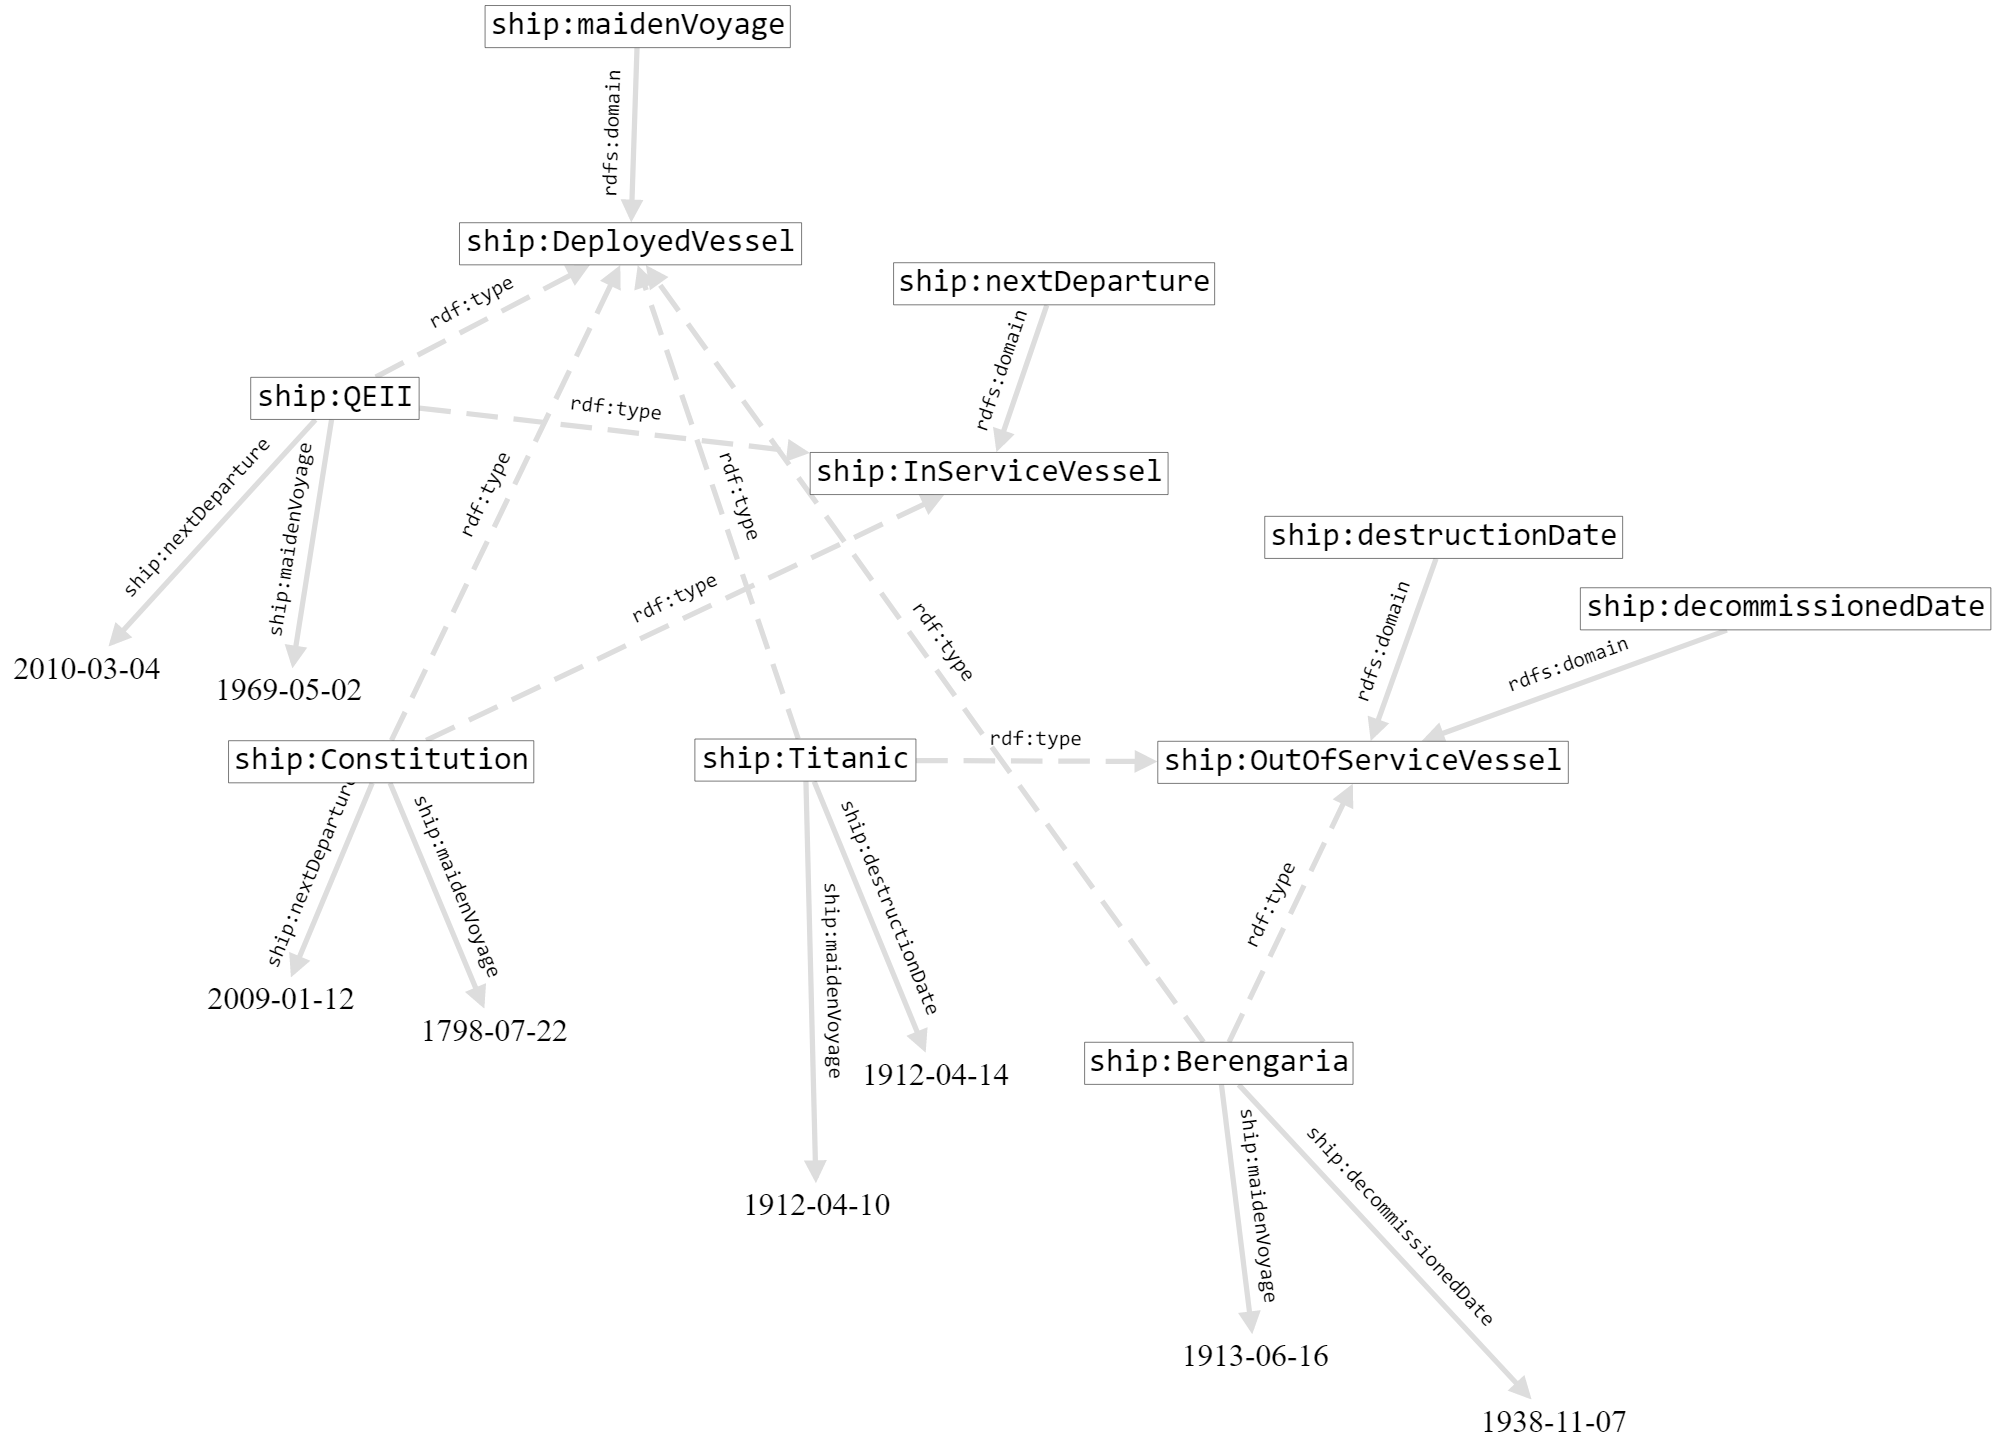
\includegraphics[width=5in]{SWWOv3/media/ch8/figure8-3.png}
\caption{Inferring classes of vessels from the information known about them.}
\label{fig:ch8.3}
\end{figure}


From the information in Table\ref{tab:ch8.1}, we can infer that all of Johnson,
Warwick, Smith, and Preble are members of the class \texttt{ship:Captain}. These
inferences, as well as the triples that led to them, can be seen in
Figure\ref{fig:ch8.4}.

\begin{figure}
\centering
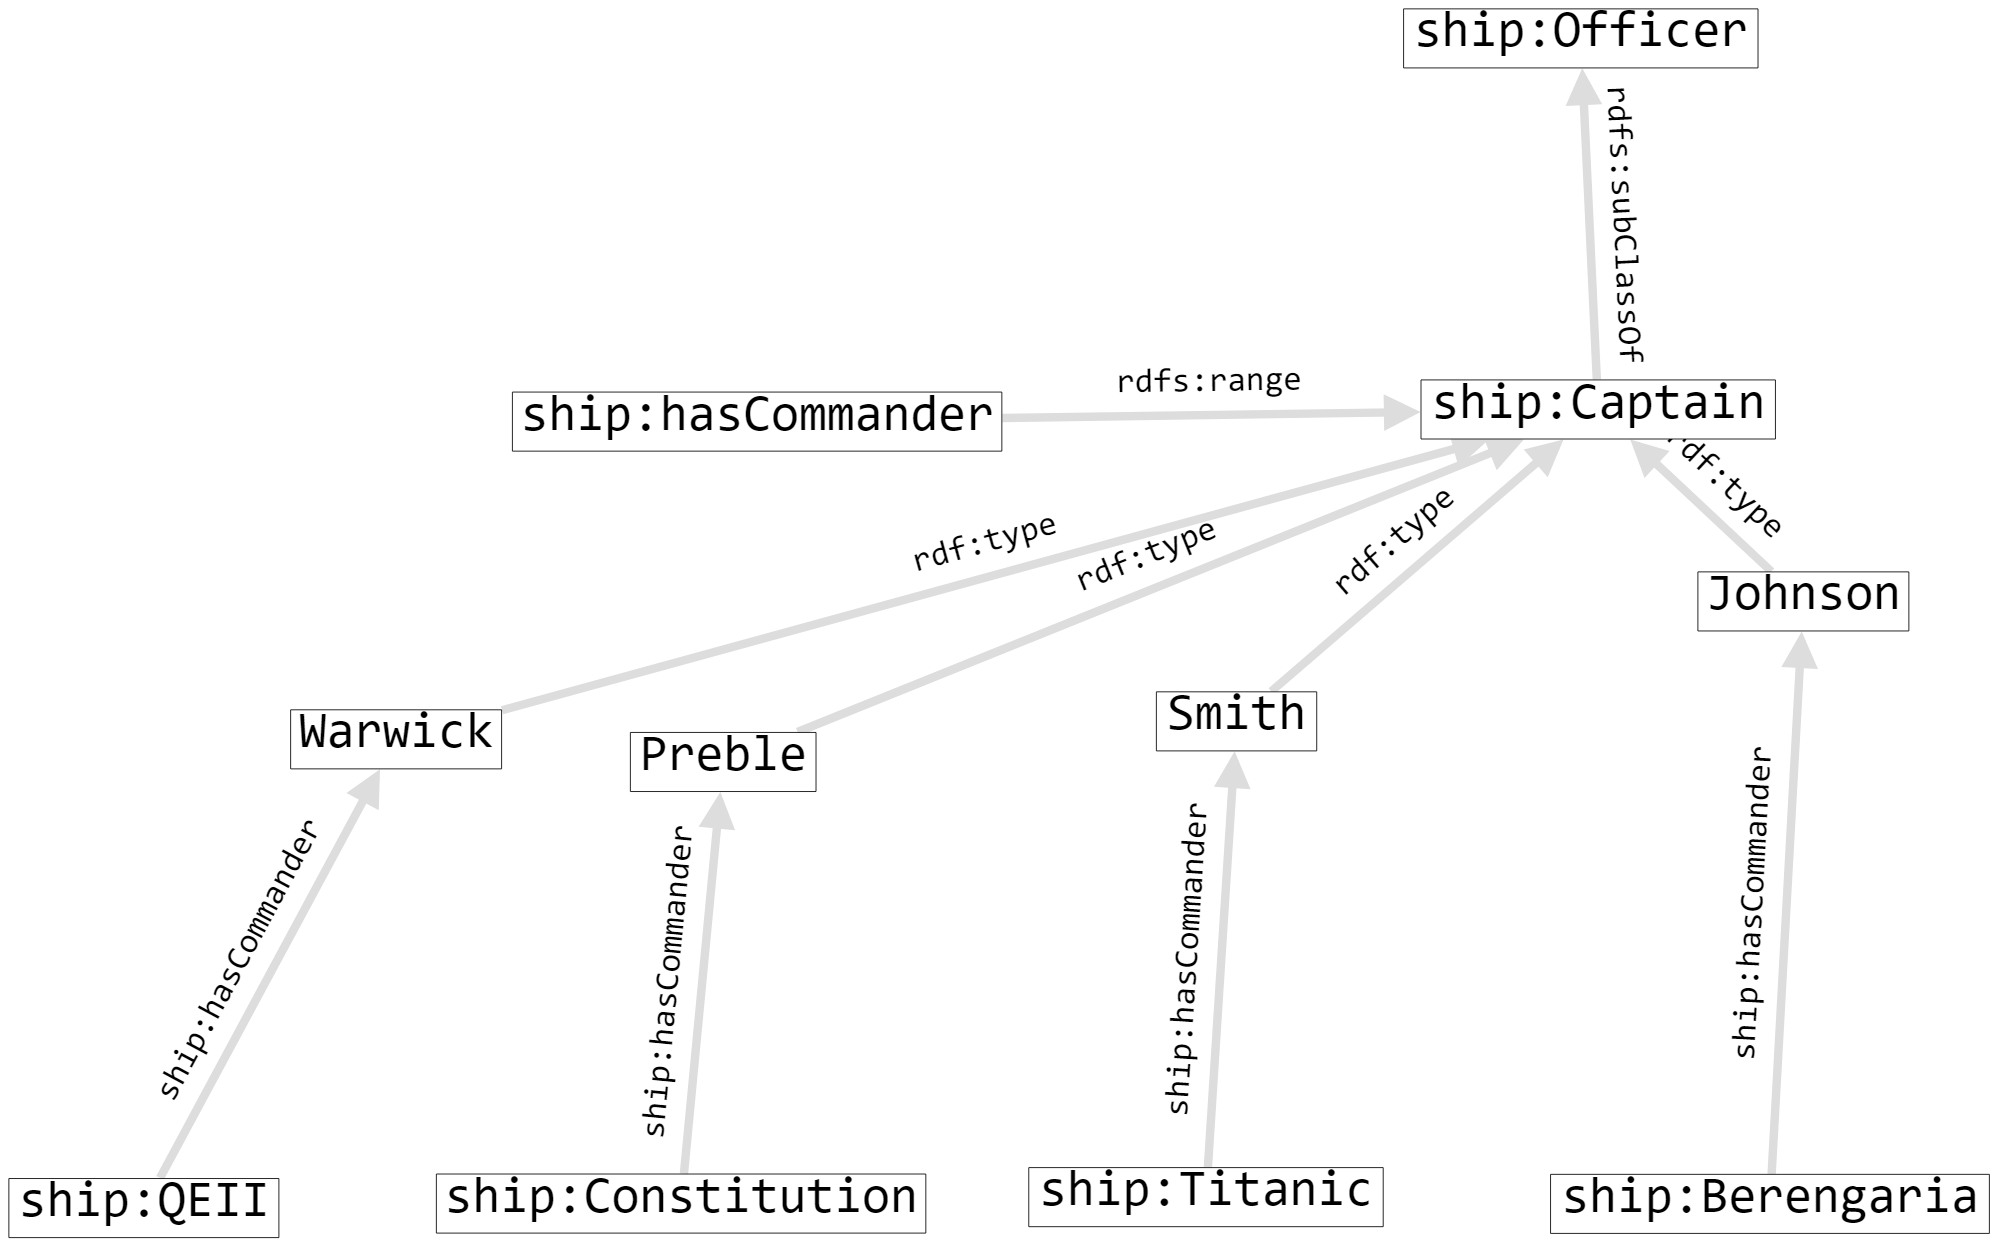
\includegraphics[width=5in]{SWWOv3/media/ch8/figure8-4.png}
\caption{Inferring that the commanders of the ships have rank "Captain"}
\label{fig:ch8.4}
\end{figure}


\end{challenge}

\subsection{Filtering undefined data}

A related challenge is to sort out individuals based on the information
that is defined for them. The set of individuals for which a particular
value is defined should be made available for future processing; those
for which it is undefined should not be processed.

\begin{challenge}{Filtering on undefined data}
\label{chal:12}

In the preceding example, the set of vessels for which \texttt{nextDeparture} is
defined could be used as input to a scheduling system that plans group
tours. Ships for which no \texttt{nextDeparture} is known should not be
considered.

\solution

It is easy to define the set of vessels that have \texttt{nextDeparture}
specified by using \texttt{rdfs:domain}. First, define a class of
\texttt{DepartingVessels} that will have these vessels as its members. Then
define this to be the domain of \texttt{nextDeparture}:

\begin{lstlisting}
ship:DepartingVessel rdf:type rdfs:Class .
ship:nextDeparture rdfs:domain ship:DepartingVessel .
\end{lstlisting}

From Table\ref{tab:ch8.1}, only the Constitution and the QEII are members of the
class 
\texttt{ship:DepartingVessels} and can be used by a scheduling program (see
Figure~\ref{fig:ch8.5}).
\end{challenge}

\subsection{RDFS and knowledge discovery}

The use of \texttt{rdfs:domain} and \texttt{rdfs:range} differs dramatically from similar
notions in other modeling paradigms. Because of the inference-based
semantics of RDFS (and OWL), domains and ranges are not used to validate
information (as is the case, for example, in OO modeling and XML) but
instead are used to determine new information based on old information.
We have just seen how this unique aspect of \texttt{rdfs:domain} and \texttt{rdfs:range}
supports particular uses of filtering and classifying information.

These definitions are among the most difficult for beginning Semantic
Web modelers to come to terms with. It is common for beginning modelers
to find these tools clumsy and difficult to use. This difficulty can be
ameliorated to some extent by understanding that RDFS in general, and
domain and range in particular, are best understood as tools for
knowledge discovery rather than knowledge description. On the Semantic
Web, we don't know in advance how information from somewhere else
on the Web should be interpreted in a new context. The RDFS definitions
of domain and range
allow us to discover new things about our data based on its use.


\begin{figure}
\centering
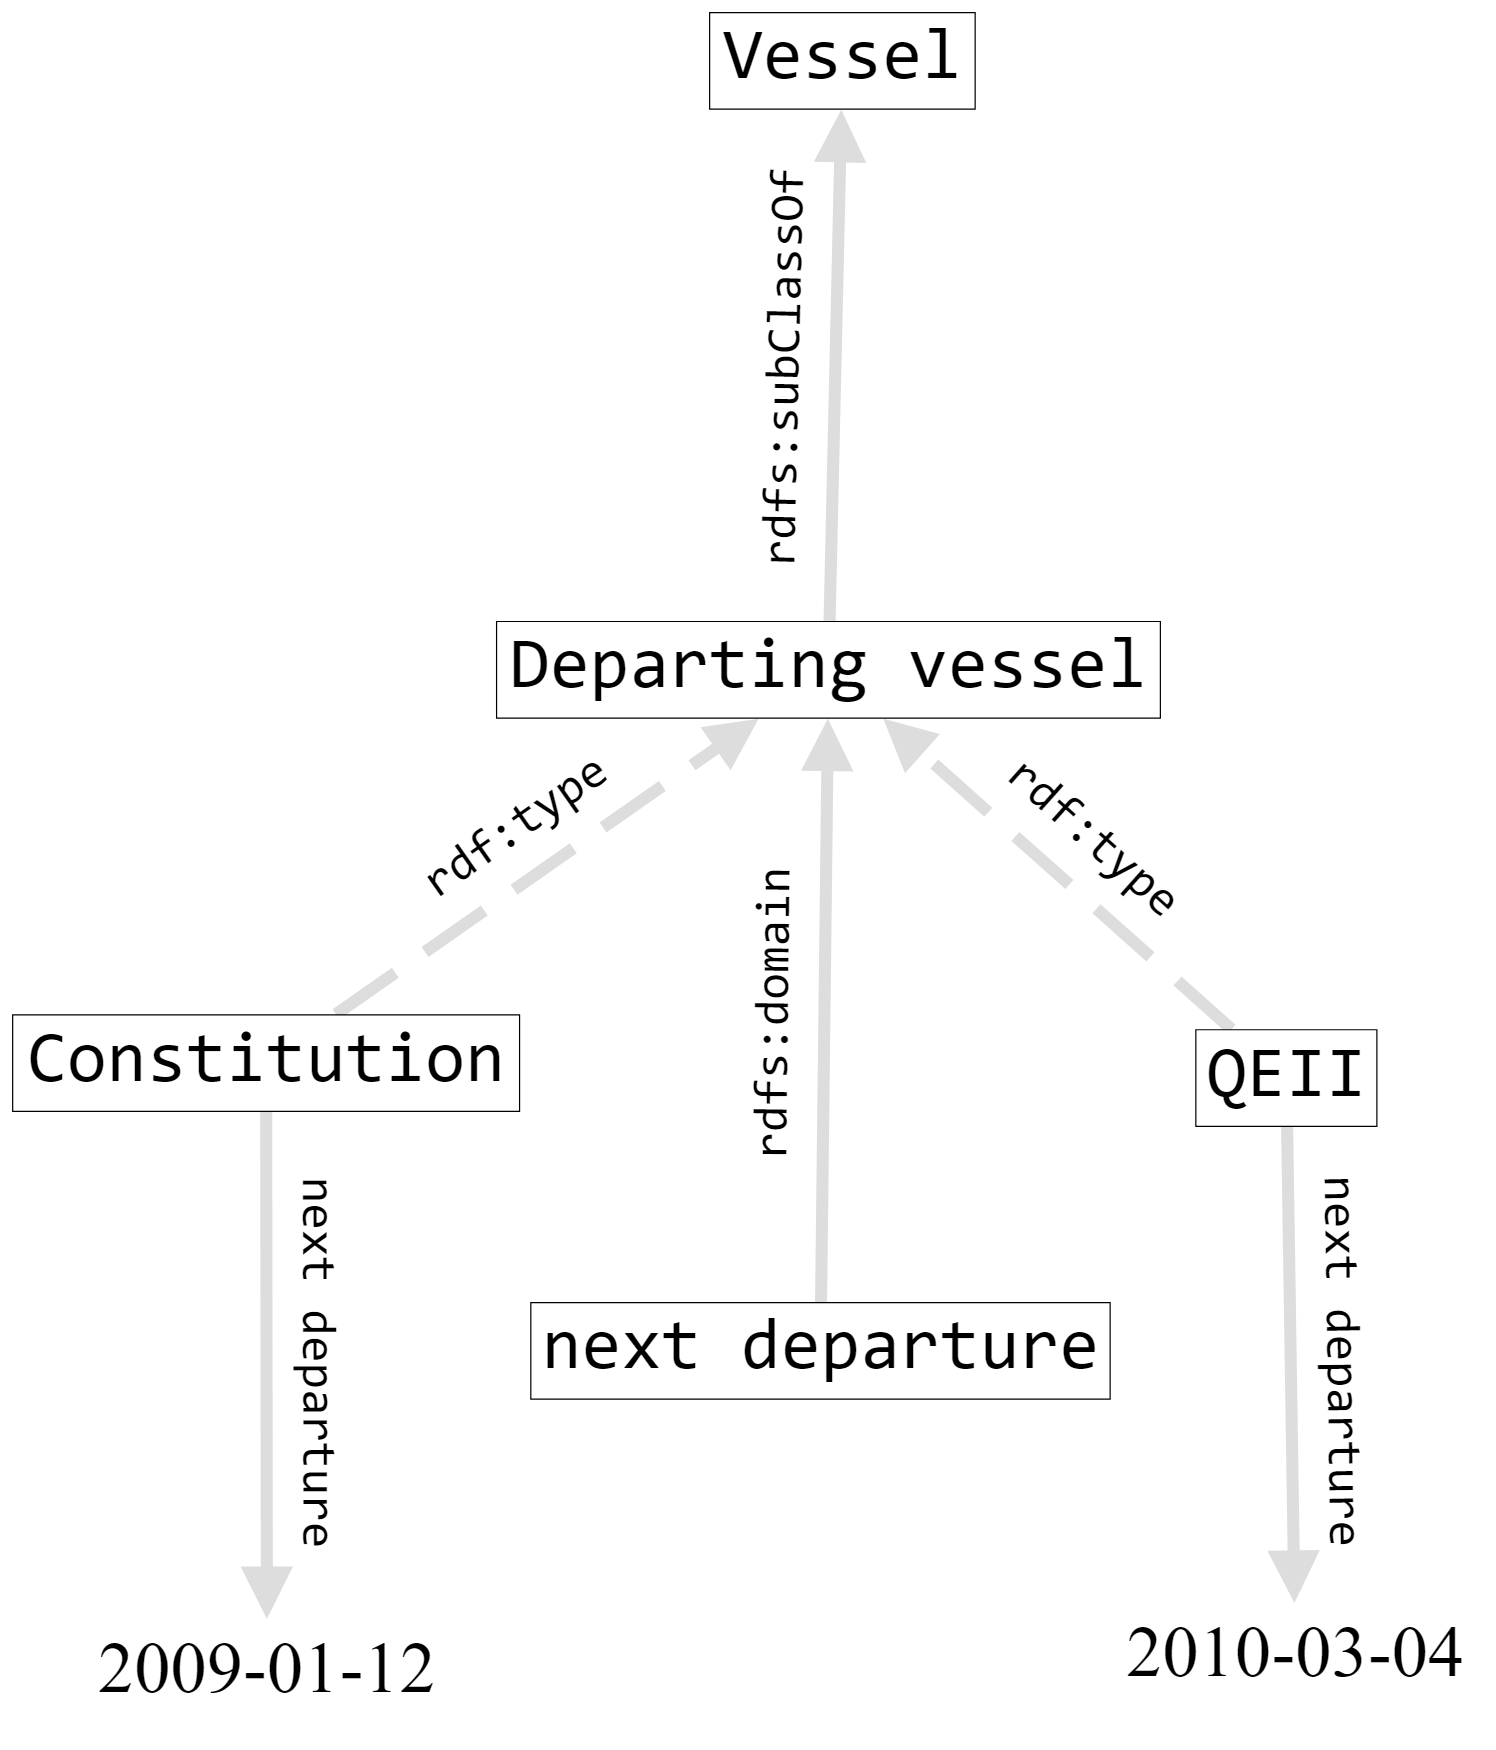
\includegraphics[width=5in]{SWWOv3/media/ch8/figure8-5.png}
\caption{Ships with a nextDeparture specified are DepartingVessels.}
\label{fig:ch8.5}
\end{figure}





What does this mean for the skillful use of domain and range in RDFS?
They are not to be used lightly---that is, merely as a way to bundle
together several properties around a class. Filtering results such as
those shown in these challenge problems are the result of the use of
domain and range. Proper use of domain and range must take these results
into account. Recommended use of domain and range goes one step further;
its use is in one of these patterns, where some particular knowledge
filtering or discovery pattern is intended. When used in this way (e.g.,
using domain to describe which of the ships are departing), it is
guaranteed that the meaning of domain and range will be appropriate even
in a web setting.

\section{Modeling with Domains and Ranges}

Although RDFS has considerable applicability in data amalgamation and
the simplicity of its small number of axioms makes it compact and easy
to implement, there are some confusions that arise even in very simple
modeling situations when using RDFS.

\subsection{Multiple domains/ranges}
\label{multidomain}
In our shipping example, we had two definitions for the \texttt{nextDeparture}
domain:

\begin{lstlisting}
ship:nextDeparture rdfs:domain DepartingVessel .
ship:nextDeparture rdfs:domain InServiceVessel .
\end{lstlisting}

What is the interpretation of these two statements? Is the \texttt{nextDeparture}
domain \texttt{DepartingVessel}, \texttt{InServiceVessel}, or both? What does this sort of
construction mean?

The right way to understand what a statement or set of statements means
in RDFS is to understand what inferences can be drawn from them. Let's
consider the case of the QEII, for which we have the following asserted
triples:

\begin{lstlisting}
ship:QEII ship:maidenVoyage "May 2, 1969" .
ship:QEII ship:nextDeparture "Mar 4, 2010" .
ship:QEII ship:hasCommander Warwick .
\end{lstlisting}

The rules of inference for \texttt{rdfs:domain} allow us to draw the following
conclusions:

\begin{lstlisting}
ship:QEII rdf:type ship:DepartingVessel.
ship:QEII rdf:type ship:InServiceVessel.
\end{lstlisting}

Each of these conclusions is drawn from the definition of \texttt{rdfs:domain},
as applied, respectively, to each of the domain declarations just given.
This behavior is not a result of a discussion of ``what will happen when
there are multiple domain statements?'' but rather a simple logical
conclusion based on the definition of \texttt{rdfs:domain}.

How can we interpret these results? Any vessel for which a \texttt{nextDeparture}
is specified will be
inferred to be a member (i.e., \texttt{rdf:type}) of both \texttt{DepartingVessel} and
\texttt{InServiceVessel} classes. Effectively, any such vessel will be inferred
to be in the intersection of the two classes specified in the domain
statements. This is something that many people find counterintuitive,
even though it is ``correct'' in RDFS.

In object-oriented modeling, when one asserts that a property (or field,
or variable, or slot) is associated with a class (as is done by
\texttt{rdfs:domain}), the intuition is that ``it is now permissible to use this
property to describe members of this class.'' If there are two such
statements, then the intuitive interpretation is that ``it is now
permissible to use this property with members of either of these
classes.'' Effectively, multiple domain declarations are interpreted in
the sense of set union: You may now use this property to describe any
item in the union of the two specified domains. For someone coming in
with this sort of expectation, the intersection behavior of RDFS can be
something of a surprise.

This interaction makes it necessary to exercise some care when modeling
information with the expectation that it will be merged with other
information. Let's suppose we have another modeling context in which a
company is managing a team of traveling salespeople. Each salesperson
has a schedule of business trips. Some of the triples that define this
model are as follows:

\begin{lstlisting}
sales:SalesPerson rdfs:subClassOf foaf:Person.
sales:sells rdfs:domain sales:SalesPerson.
sales:sells rdfs:range sales:ProductLine.
sales:nextDeparture rdfs:domain sales:SalesPerson.
\end{lstlisting}

That is, we have a sales force that covers certain \texttt{ProductLines}; each
member travels on a regular basis, and it is useful for us to track the
date of the next departure of any particular \texttt{SalesPerson}.

Suppose we were to merge the information for our sales force management
with the schedules of
the ocean liners. This merge becomes interesting if we map some of the
items in one model to items
in another. An obvious candidate for such a mapping is between
\texttt{sales:nextDeparture} and \texttt{ship:nextDeparture}. Both refer to dates, and the
intuition is that they specify the next departure date of something or
someone. So a simple connection to make between the two models would be
to link these two properties, such as the following:

\begin{lstlisting}
sales:nextDeparture rdfs:subPropertyOf ship:nextDeparture.
ship:nextDeparture rdfs:subPropertyOf sales:nextDeparture.
\end{lstlisting}

using the mutual \texttt{subPropertyOf} pattern. The intuition here is that the
two uses of
\texttt{nextDeparture}, one for ships and the other for sales, are in fact the
same.

But wait! Let's see what inferences are drawn from this merger. Suppose
we have a triple that describes a member of the sales force:

\begin{lstlisting}
sales:Johannes sales:nextDeparture "May 31, 2008".
\end{lstlisting}

and we already have the triple about the QEII:

\begin{lstlisting}
ship:QEII ship:nextDeparture "Mar 4, 2010".
\end{lstlisting}

What inferences can we draw from these two triples? Using
\texttt{rdfs:subPropertyOf} inferences first, then \texttt{rdfs:domain} inferences, and
finally using the \texttt{rdfs:subClassO}f triple with \texttt{foaf:Person}, we get the
following inferred triples:

\begin{lstlisting}
* sales:Johannes ship:nextDeparture "May 31, 2008".
* ship:QEII sales:nextDeparture "Mar 4, 2010".
* sales:Johannes rdf:type ship:DepartingVessel.
* ship:QEII rdf:type sales:SalesPerson.
* ship:QEII rdf:type foaf:Person.
\end{lstlisting}


These inferences start off innocently enough, but they become more and
more counterintuitive as they go on, and eventually (when the QEII is
classified as a \texttt{foaf:Person}) become completely outrageous (or perhaps
dangerously misleading, especially given that the Monarch herself might
actually be a \texttt{foaf:Person}, causing the inferences to confuse the Monarch
with the ship named after her). The asserted triples, and the inferences
that can be drawn from them, are shown in Figure~\ref{fig:ch8.6}.

It is easy to lay blame for this unfortunate behavior at the feet of the
definition of \texttt{rdfs:domain}, but to do so would throw out the baby with
the bathwater. The real issue in this example is that we have made a
modeling error. The error resulted from the overzealous urge to jump to
the conclusion that two properties should be mapped so closely to each
other. The ramifications of using \texttt{subPropertyOf} (or any other RDFS
construct) can be subtle and far-reaching.

In particular, when each of these models stated its respective domain
and range statements about \texttt{sales:nextDeparture} and \texttt{ship:nextDeparture},
respectively, it was saying, ``Whenever you see any individual described
by \texttt{sales:nextDeparture} (resp. \texttt{ship:nextDeparture}), that individual is
known to be of type \texttt{sales:SalesPerson} (resp. \texttt{ship:DepartingVessel}).''
This is quite a strong statement, and it should be treated as such. In
particular, it would be surprising if two properties defined so
specifically would not have extreme ramifications when merged.

\begin{figure}
\centering
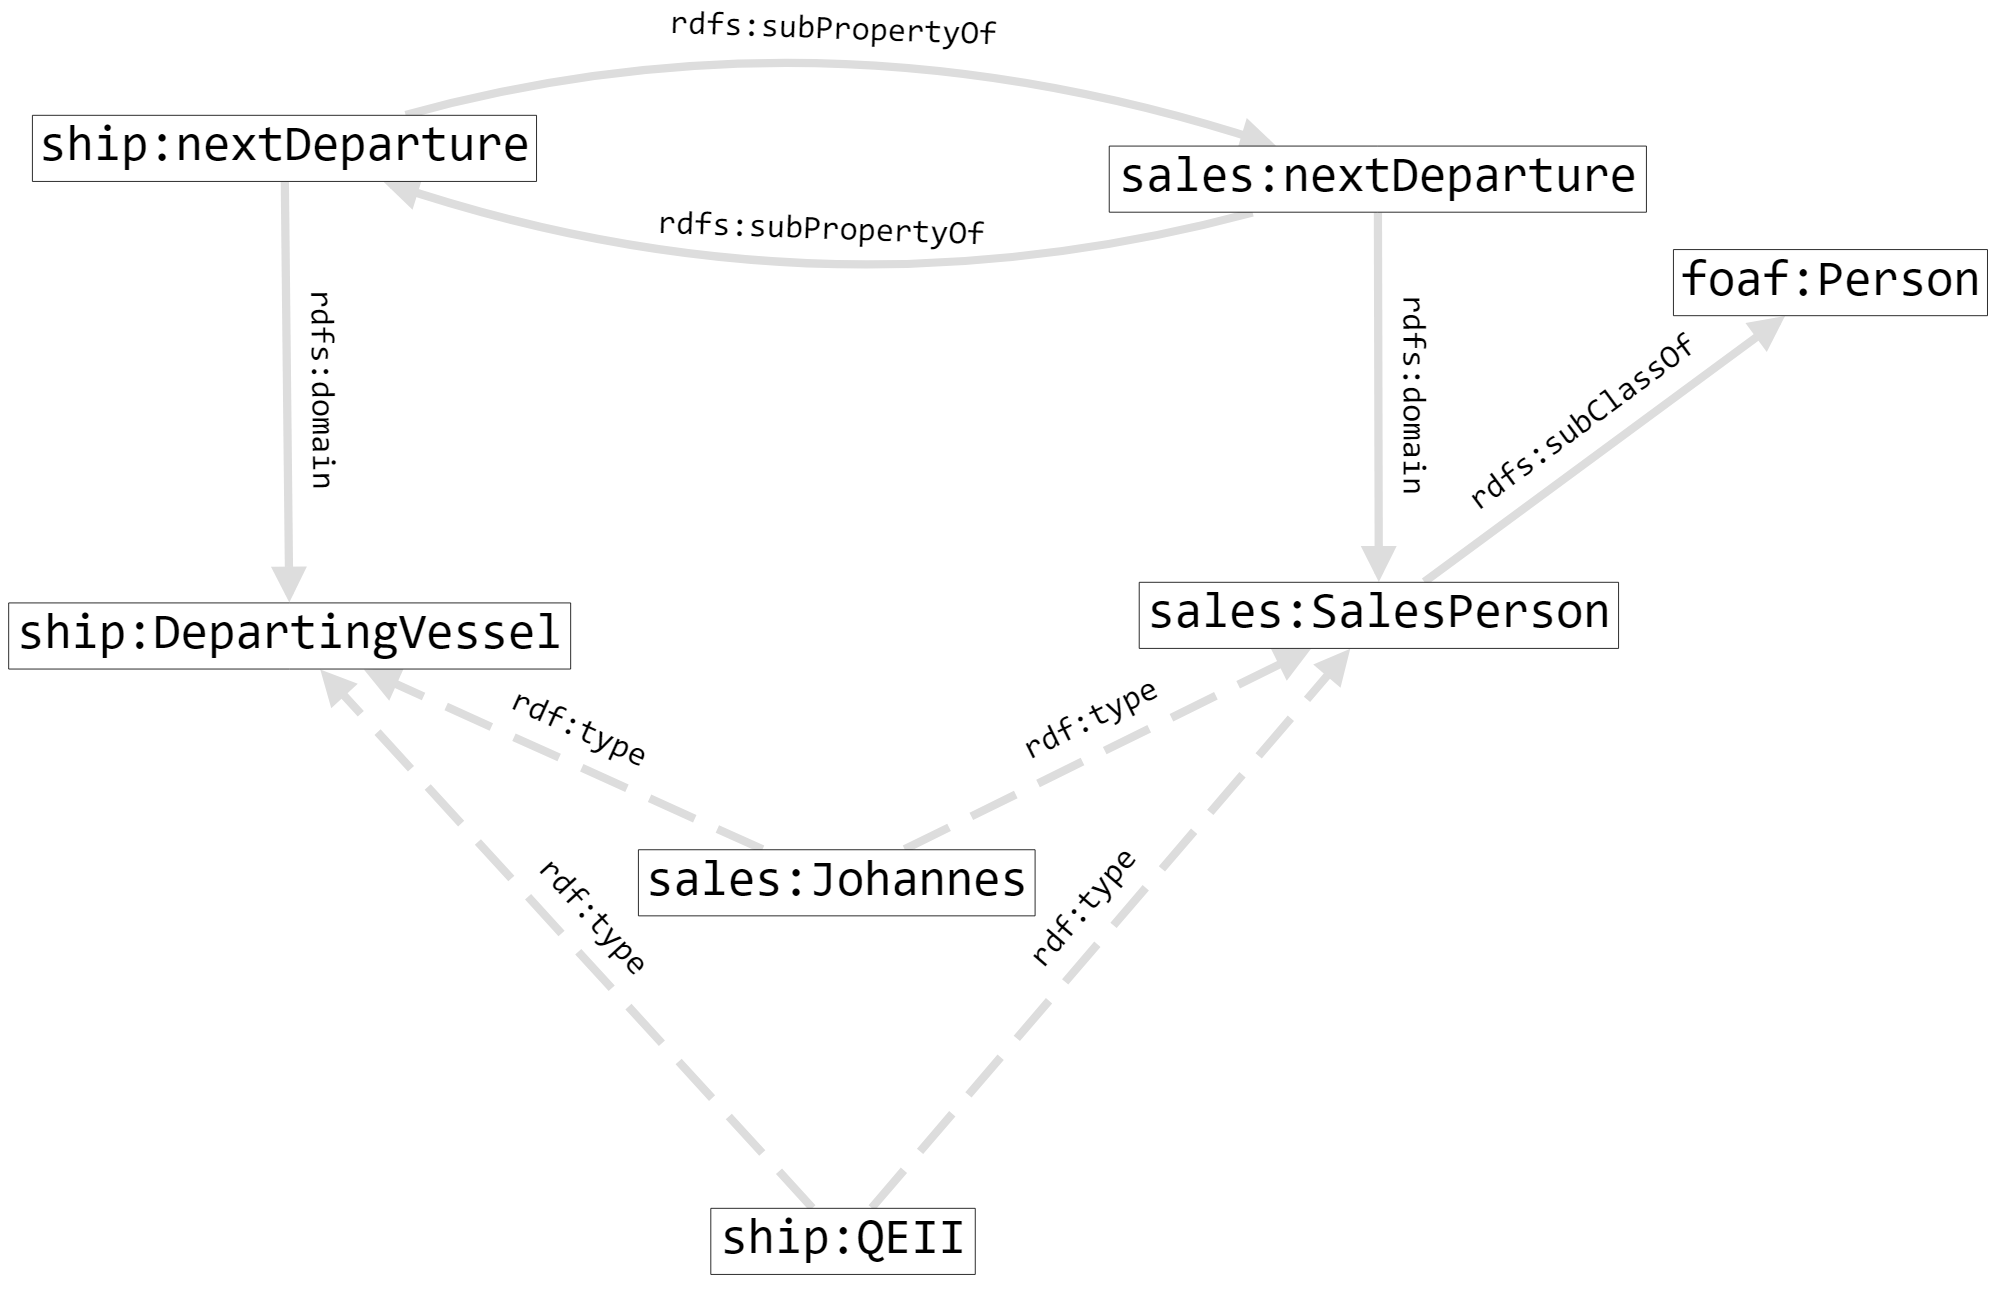
\includegraphics[width=5in]{SWWOv3/media/ch8/figure8-6.png}
\caption{Inferences resulting from merging two notions of nextDeparture.}
\label{fig:ch8.6}
\end{figure}



So what is the solution? Should we refrain from merging properties? This
is hardly a solution in the spirit of the Semantic Web. Should we avoid
making strong statements about properties? This will not help us to make
useful models. Should we change the RDFS standard so we can't make these
statements? This is a bit extreme, but as we shall see, OWL does provide
some more subtle constructs for property definitions that allow for
finer-grained modeling. Rather, the solution lies in understanding the
source of the modeling error that is at the heart of this example: We
should refrain from merging things, like the two notions of
\texttt{nextDeparture}, whose meanings have important differences.

Using the idioms and patterns of RDFS shown in this chapter, there are
more things we can do, depending on our motivation for the merger. In
particular, we can still merge these two properties but without making
such a strong statement about their equivalence.

If, for instance, we just want to merge the two notions of \texttt{nextDeparture}
to drive a calendar application that shows all the departure dates for
the sales force and the ocean liner fleet, then what we really want is a
single property that will provide us the information we need (as we did
in the property union pattern). Rather than mapping the properties from
one domain to another, instead we map both properties to a third,
domain-neutral property, thus:

\begin{lstlisting}
ship:nextDeparture rdfs:subPropertyOf cal:nextDeparture .
sales:nextDeparture rdfs:subPropertyOf cal:nextDeparture .
\end{lstlisting}

Notice that the amalgamating property \texttt{cal:nextDeparture} doesn't need any
domain information at all. After all, we don't need to make any
(further) inferences about the types of the entities that it is used to
describe. Now we can infer that

\begin{lstlisting}
* sales:Johannes cal:nextDeparture "May 31, 2008" .
* ship:QEII cal:nextDeparture "Mar 4, 2010" .
\end{lstlisting}

A single calendar display, sorted by the property \texttt{cal:nextDeparture},
will show these two dates, but no further inference can be made. In
particular, no inferences will be made about considering the QEII as a
member of the sales force or Johannes as a sailing vessel.

This behavior of RDFS is not an idiosyncrasy of how it was defined, it is
a direct result of the fact that on the Semantic Web, we are representing distributed
data, and that includes distributed metadata.  Each stakeholder is telling us 
something about one of their properties (in this example, \texttt{ship:nextDeparture} and
\texttt{sales:nextDeparture}).  We need to be able to draw conclusions from 
each of these things in their own context.  But when we combine them (as 
we did, when we asserted that they were sub properties of one another), now we 
have to accept both definitions together.  This isn't an arbitrary decision on 
the part of the RDF design; it is simply a ramification of treating the statements
from each contributor equally.  If we believe what the Sales domain says, and we believe
what the Ship domain says, and if we believe our mapping, then the domain must 
be the intersection of the stated domains.   When we resolve this situation (e.g., by
making a new property, \texttt{cal:nextDeparture} that encompasses both of these properties
we are being specific about the relationship between them.  This is what we have to
do, to be able to use both data sources together. 

This is the art of modeling in the Semantic Web; to state specifically and in sufficient 
detail how two or more data sets (or metadata sets) are related.  The inference model
behind languages like RDFS and OWL provide the precision we need to build this kind of model. 



\section{Nonmodeling Properties in RDFS}

In addition to the properties described so far, RDFS also provides a
handful of properties that have no defined inference semantics---that
is, there are no inferences that derive from them. We already saw one
example of such a property, \texttt{rdfs:label}. No inferences are drawn from
\texttt{rdfs:label}, so in that sense it has no semantics. Nevertheless, it does
by convention have an operational semantics in that it describes the
ways in which display agents interact with the model.

\subsection{Cross-referencing files: rdfs:seeAlso}

Every resource in a Semantic Web model is specified by a URI that can
also be dereferenced and used as a URL. In the case where this URL
resolves to a real document, this provides a place where defining
information about a resource can be stored.

In some contexts, it is useful to include some supplementary information
about a resource for its use in a certain context. This is usually meant
to be other documents that might help explain the entity---for example,
we might include a pointer to a Wikipedia entry, or a pointer to related
data (e.g., if the resource corresponds to a table from a database, the
supplementary information could be the other tables from the same
database) or even to another RDF or RDFS file that contains linked
information. For such cases, \texttt{rdfs:seeAlso} provides a way to specify the
web location of this supplementary information (i.e. it should be a URI,
not a human-readable property). \texttt{rdfs:seeAlso} has no formal semantics, so
the precise behavior of any processor when it encounters \texttt{rdfs:seeAlso} is
not specified. A common behavior of tools that encounter \texttt{rdfs:seeAlso}
links is to expose those links in a browser or application interface
through which the RDFS document is being used.

\subsection{Organizing vocabularies: rdfs:isDefinedBy}

Just as \texttt{rdfs:seeAlso} can provide supplementary information about a
resource, \texttt{rdfs:isDefinedBy} provides a link to the primary source of
information about a resource. This allows modelers to specify where the
definitional description of a resource can be found. \texttt{rdfs:isDefinedBy} is
defined in RDF to be a \texttt{rdfs:subPropertyOf} of \texttt{rdfs:seeAlso}.

\subsection{Model documentation: rdfs:comment}

Just as in any computer language (modeling languages, markup languages,
or programming languages), sometimes it is helpful if a document author
can leave natural language comments about a model for future readers to
see. Since RDFS is implemented entirely in RDF, the comment feature is
also implemented in RDF. To make a comment on some part of a model,
simply assert a triple using the property \texttt{rdfs:comment} as a predicate.
A good practice is also to indicate the natural language used to support 
internationalization of data, applications and interfaces, as follows:

\begin{lstlisting}
sales:nextDeparture rdfs:comment
   "This indicates the next planned departure date for a salesperson."@en ,
   "Ceci indique la prochaine date de d(*@\'e@*)part pr(*@\'e@*)vue pour un vendeur."@fr .
\end{lstlisting}

\section{SUMMARY}

RDFS is the schema language for RDF; it describes constructs for types
of objects (Classes), relating types to one another (subClasses),
properties that describe objects (Properties), and relationships between
them (subProperty). The Class system in RDFS includes a simple and
elegant notion of inheritance, based on set inclusion; one class is a
subclass of another means that instances of the one are also instances
of the other.

The RDFS language benefits from the distributed nature of RDF and all
its tools by being expressed in RDF itself. All schema information
(classes, subclasses, subproperties, domain, range, etc.) is expressed
in RDF triples. In particular, this makes schema information, as well as
data, subject to the AAA slogan: Anyone can say Anything about Any
topic---even about the schema.

The semantics of RDFS is expressed through the mechanism of inferencing;
that is, the meaning of any construct in RDFS is given by the inferences
that can be inferred from it. For example, it is this simple but
powerful mechanism for specifying semantics that allows for the short
and elegant defi- nition of subclass and subproperty.

RDFS also includes the constructs \texttt{rdfs:domain} and \texttt{rdfs:range} to describe
the relationship between properties and classes. The meanings of these
constructs are given by very simple rules, but these rules have subtle
and far-reaching impact. The rules may be simple, but the statements are
powerful.

Even with its small set of constructs and simple rules, RDFS allows for
the resolution of a wide variety of integration issues. Whenever you
might think of doing a global find-and-replace in a set of structured
data, consider using \texttt{rdfs:subPropertyOf} or \texttt{rdfs:subClassOf} instead. It
may seem trivial to say that one should merge only entities from
multiple sources that don't have important differences. Using the
inference mechanism of RDFS, we can determine just what happens when we
do merge things and judge whether the results are desirable or
dangerous. Although RDFS does not provide logical primitives like union
and intersection, it is often possible to achieve desired inferences by
using specific patterns of \texttt{subClassOf} and \texttt{subPropertyOf}. RDFS provides a
framework through which information can flow; we can think of \texttt{subClassOf}
and \texttt{subPropertyOf} as the IF/ THEN facility of semantic modeling. This
utility persists even when we move on to modeling in OWL. In fact, using
\texttt{subClassOf} in this way provides a cornerstone of OWL modeling.

When used in careful combination, the constructs of RDFS are
particularly effective at defining

how differently structured information can be used together in a uniform
way.

\subsection{Fundamental concepts}

The following fundamental concepts were introduced in this chapter.

rdfs:subClassOf---Relation between classes, that the members of one
class are included in the members of the other.

rdfs:subPropertyOf---Relation between properties, that the pairs related
by one property are included in the other.

rdfs:domain and rdfs:range---Description of a property that determines
class membership
of individuals related by that property.

Logical operations (Union, Intersection, etc.) in RDFS---RDFS constructs
can be used to simulate certain logical combinations of sets and
properties.
